
\documentclass{article}
\usepackage{graphicx, color}
\newcommand{\hlnumber}[1]{\textcolor[rgb]{0,0,0}{#1}}%
\newcommand{\hlfunctioncall}[1]{\textcolor[rgb]{.5,0,.33}{\textbf{#1}}}%
\newcommand{\hlstring}[1]{\textcolor[rgb]{.6,.6,1}{#1}}%
\newcommand{\hlkeyword}[1]{\textbf{#1}}%
\newcommand{\hlargument}[1]{\textcolor[rgb]{.69,.25,.02}{#1}}%
\newcommand{\hlcomment}[1]{\textcolor[rgb]{.18,.6,.34}{#1}}%
\newcommand{\hlroxygencomment}[1]{\textcolor[rgb]{.44,.48,.7}{#1}}%
\newcommand{\hlformalargs}[1]{\hlargument{#1}}%
\newcommand{\hleqformalargs}[1]{\hlargument{#1}}%
\newcommand{\hlassignement}[1]{\textbf{#1}}%
\newcommand{\hlpackage}[1]{\textcolor[rgb]{.59,.71,.145}{#1}}%
\newcommand{\hlslot}[1]{\textit{#1}}%
\newcommand{\hlsymbol}[1]{#1}%
\newcommand{\hlprompt}[1]{\textcolor[rgb]{.5,.5,.5}{#1}}%

\usepackage{color}%
 
\newsavebox{\hlnormalsizeboxclosebrace}%
\newsavebox{\hlnormalsizeboxopenbrace}%
\newsavebox{\hlnormalsizeboxbackslash}%
\newsavebox{\hlnormalsizeboxlessthan}%
\newsavebox{\hlnormalsizeboxgreaterthan}%
\newsavebox{\hlnormalsizeboxdollar}%
\newsavebox{\hlnormalsizeboxunderscore}%
\newsavebox{\hlnormalsizeboxand}%
\newsavebox{\hlnormalsizeboxhash}%
\newsavebox{\hlnormalsizeboxat}%
\newsavebox{\hlnormalsizeboxpercent}% 
\newsavebox{\hlnormalsizeboxhat}%
\newsavebox{\hlnormalsizeboxsinglequote}%
\newsavebox{\hlnormalsizeboxbacktick}%

\setbox\hlnormalsizeboxopenbrace=\hbox{\begin{normalsize}\verb.{.\end{normalsize}}%
\setbox\hlnormalsizeboxclosebrace=\hbox{\begin{normalsize}\verb.}.\end{normalsize}}%
\setbox\hlnormalsizeboxlessthan=\hbox{\begin{normalsize}\verb.<.\end{normalsize}}%
\setbox\hlnormalsizeboxdollar=\hbox{\begin{normalsize}\verb.$.\end{normalsize}}%
\setbox\hlnormalsizeboxunderscore=\hbox{\begin{normalsize}\verb._.\end{normalsize}}%
\setbox\hlnormalsizeboxand=\hbox{\begin{normalsize}\verb.&.\end{normalsize}}%
\setbox\hlnormalsizeboxhash=\hbox{\begin{normalsize}\verb.#.\end{normalsize}}%
\setbox\hlnormalsizeboxat=\hbox{\begin{normalsize}\verb.@.\end{normalsize}}%
\setbox\hlnormalsizeboxbackslash=\hbox{\begin{normalsize}\verb.\.\end{normalsize}}%
\setbox\hlnormalsizeboxgreaterthan=\hbox{\begin{normalsize}\verb.>.\end{normalsize}}%
\setbox\hlnormalsizeboxpercent=\hbox{\begin{normalsize}\verb.%.\end{normalsize}}%
\setbox\hlnormalsizeboxhat=\hbox{\begin{normalsize}\verb.^.\end{normalsize}}%
\setbox\hlnormalsizeboxsinglequote=\hbox{\begin{normalsize}\verb.'.\end{normalsize}}%
\setbox\hlnormalsizeboxbacktick=\hbox{\begin{normalsize}\verb.`.\end{normalsize}}%
\setbox\hlnormalsizeboxhat=\hbox{\begin{normalsize}\verb.^.\end{normalsize}}%



\newsavebox{\hltinyboxclosebrace}%
\newsavebox{\hltinyboxopenbrace}%
\newsavebox{\hltinyboxbackslash}%
\newsavebox{\hltinyboxlessthan}%
\newsavebox{\hltinyboxgreaterthan}%
\newsavebox{\hltinyboxdollar}%
\newsavebox{\hltinyboxunderscore}%
\newsavebox{\hltinyboxand}%
\newsavebox{\hltinyboxhash}%
\newsavebox{\hltinyboxat}%
\newsavebox{\hltinyboxpercent}% 
\newsavebox{\hltinyboxhat}%
\newsavebox{\hltinyboxsinglequote}%
\newsavebox{\hltinyboxbacktick}%

\setbox\hltinyboxopenbrace=\hbox{\begin{tiny}\verb.{.\end{tiny}}%
\setbox\hltinyboxclosebrace=\hbox{\begin{tiny}\verb.}.\end{tiny}}%
\setbox\hltinyboxlessthan=\hbox{\begin{tiny}\verb.<.\end{tiny}}%
\setbox\hltinyboxdollar=\hbox{\begin{tiny}\verb.$.\end{tiny}}%
\setbox\hltinyboxunderscore=\hbox{\begin{tiny}\verb._.\end{tiny}}%
\setbox\hltinyboxand=\hbox{\begin{tiny}\verb.&.\end{tiny}}%
\setbox\hltinyboxhash=\hbox{\begin{tiny}\verb.#.\end{tiny}}%
\setbox\hltinyboxat=\hbox{\begin{tiny}\verb.@.\end{tiny}}%
\setbox\hltinyboxbackslash=\hbox{\begin{tiny}\verb.\.\end{tiny}}%
\setbox\hltinyboxgreaterthan=\hbox{\begin{tiny}\verb.>.\end{tiny}}%
\setbox\hltinyboxpercent=\hbox{\begin{tiny}\verb.%.\end{tiny}}%
\setbox\hltinyboxhat=\hbox{\begin{tiny}\verb.^.\end{tiny}}%
\setbox\hltinyboxsinglequote=\hbox{\begin{tiny}\verb.'.\end{tiny}}%
\setbox\hltinyboxbacktick=\hbox{\begin{tiny}\verb.`.\end{tiny}}%
\setbox\hltinyboxhat=\hbox{\begin{tiny}\verb.^.\end{tiny}}%



\newsavebox{\hlscriptsizeboxclosebrace}%
\newsavebox{\hlscriptsizeboxopenbrace}%
\newsavebox{\hlscriptsizeboxbackslash}%
\newsavebox{\hlscriptsizeboxlessthan}%
\newsavebox{\hlscriptsizeboxgreaterthan}%
\newsavebox{\hlscriptsizeboxdollar}%
\newsavebox{\hlscriptsizeboxunderscore}%
\newsavebox{\hlscriptsizeboxand}%
\newsavebox{\hlscriptsizeboxhash}%
\newsavebox{\hlscriptsizeboxat}%
\newsavebox{\hlscriptsizeboxpercent}% 
\newsavebox{\hlscriptsizeboxhat}%
\newsavebox{\hlscriptsizeboxsinglequote}%
\newsavebox{\hlscriptsizeboxbacktick}%

\setbox\hlscriptsizeboxopenbrace=\hbox{\begin{scriptsize}\verb.{.\end{scriptsize}}%
\setbox\hlscriptsizeboxclosebrace=\hbox{\begin{scriptsize}\verb.}.\end{scriptsize}}%
\setbox\hlscriptsizeboxlessthan=\hbox{\begin{scriptsize}\verb.<.\end{scriptsize}}%
\setbox\hlscriptsizeboxdollar=\hbox{\begin{scriptsize}\verb.$.\end{scriptsize}}%
\setbox\hlscriptsizeboxunderscore=\hbox{\begin{scriptsize}\verb._.\end{scriptsize}}%
\setbox\hlscriptsizeboxand=\hbox{\begin{scriptsize}\verb.&.\end{scriptsize}}%
\setbox\hlscriptsizeboxhash=\hbox{\begin{scriptsize}\verb.#.\end{scriptsize}}%
\setbox\hlscriptsizeboxat=\hbox{\begin{scriptsize}\verb.@.\end{scriptsize}}%
\setbox\hlscriptsizeboxbackslash=\hbox{\begin{scriptsize}\verb.\.\end{scriptsize}}%
\setbox\hlscriptsizeboxgreaterthan=\hbox{\begin{scriptsize}\verb.>.\end{scriptsize}}%
\setbox\hlscriptsizeboxpercent=\hbox{\begin{scriptsize}\verb.%.\end{scriptsize}}%
\setbox\hlscriptsizeboxhat=\hbox{\begin{scriptsize}\verb.^.\end{scriptsize}}%
\setbox\hlscriptsizeboxsinglequote=\hbox{\begin{scriptsize}\verb.'.\end{scriptsize}}%
\setbox\hlscriptsizeboxbacktick=\hbox{\begin{scriptsize}\verb.`.\end{scriptsize}}%
\setbox\hlscriptsizeboxhat=\hbox{\begin{scriptsize}\verb.^.\end{scriptsize}}%



\newsavebox{\hlfootnotesizeboxclosebrace}%
\newsavebox{\hlfootnotesizeboxopenbrace}%
\newsavebox{\hlfootnotesizeboxbackslash}%
\newsavebox{\hlfootnotesizeboxlessthan}%
\newsavebox{\hlfootnotesizeboxgreaterthan}%
\newsavebox{\hlfootnotesizeboxdollar}%
\newsavebox{\hlfootnotesizeboxunderscore}%
\newsavebox{\hlfootnotesizeboxand}%
\newsavebox{\hlfootnotesizeboxhash}%
\newsavebox{\hlfootnotesizeboxat}%
\newsavebox{\hlfootnotesizeboxpercent}% 
\newsavebox{\hlfootnotesizeboxhat}%
\newsavebox{\hlfootnotesizeboxsinglequote}%
\newsavebox{\hlfootnotesizeboxbacktick}%

\setbox\hlfootnotesizeboxopenbrace=\hbox{\begin{footnotesize}\verb.{.\end{footnotesize}}%
\setbox\hlfootnotesizeboxclosebrace=\hbox{\begin{footnotesize}\verb.}.\end{footnotesize}}%
\setbox\hlfootnotesizeboxlessthan=\hbox{\begin{footnotesize}\verb.<.\end{footnotesize}}%
\setbox\hlfootnotesizeboxdollar=\hbox{\begin{footnotesize}\verb.$.\end{footnotesize}}%
\setbox\hlfootnotesizeboxunderscore=\hbox{\begin{footnotesize}\verb._.\end{footnotesize}}%
\setbox\hlfootnotesizeboxand=\hbox{\begin{footnotesize}\verb.&.\end{footnotesize}}%
\setbox\hlfootnotesizeboxhash=\hbox{\begin{footnotesize}\verb.#.\end{footnotesize}}%
\setbox\hlfootnotesizeboxat=\hbox{\begin{footnotesize}\verb.@.\end{footnotesize}}%
\setbox\hlfootnotesizeboxbackslash=\hbox{\begin{footnotesize}\verb.\.\end{footnotesize}}%
\setbox\hlfootnotesizeboxgreaterthan=\hbox{\begin{footnotesize}\verb.>.\end{footnotesize}}%
\setbox\hlfootnotesizeboxpercent=\hbox{\begin{footnotesize}\verb.%.\end{footnotesize}}%
\setbox\hlfootnotesizeboxhat=\hbox{\begin{footnotesize}\verb.^.\end{footnotesize}}%
\setbox\hlfootnotesizeboxsinglequote=\hbox{\begin{footnotesize}\verb.'.\end{footnotesize}}%
\setbox\hlfootnotesizeboxbacktick=\hbox{\begin{footnotesize}\verb.`.\end{footnotesize}}%
\setbox\hlfootnotesizeboxhat=\hbox{\begin{footnotesize}\verb.^.\end{footnotesize}}%



\newsavebox{\hlsmallboxclosebrace}%
\newsavebox{\hlsmallboxopenbrace}%
\newsavebox{\hlsmallboxbackslash}%
\newsavebox{\hlsmallboxlessthan}%
\newsavebox{\hlsmallboxgreaterthan}%
\newsavebox{\hlsmallboxdollar}%
\newsavebox{\hlsmallboxunderscore}%
\newsavebox{\hlsmallboxand}%
\newsavebox{\hlsmallboxhash}%
\newsavebox{\hlsmallboxat}%
\newsavebox{\hlsmallboxpercent}% 
\newsavebox{\hlsmallboxhat}%
\newsavebox{\hlsmallboxsinglequote}%
\newsavebox{\hlsmallboxbacktick}%

\setbox\hlsmallboxopenbrace=\hbox{\begin{small}\verb.{.\end{small}}%
\setbox\hlsmallboxclosebrace=\hbox{\begin{small}\verb.}.\end{small}}%
\setbox\hlsmallboxlessthan=\hbox{\begin{small}\verb.<.\end{small}}%
\setbox\hlsmallboxdollar=\hbox{\begin{small}\verb.$.\end{small}}%
\setbox\hlsmallboxunderscore=\hbox{\begin{small}\verb._.\end{small}}%
\setbox\hlsmallboxand=\hbox{\begin{small}\verb.&.\end{small}}%
\setbox\hlsmallboxhash=\hbox{\begin{small}\verb.#.\end{small}}%
\setbox\hlsmallboxat=\hbox{\begin{small}\verb.@.\end{small}}%
\setbox\hlsmallboxbackslash=\hbox{\begin{small}\verb.\.\end{small}}%
\setbox\hlsmallboxgreaterthan=\hbox{\begin{small}\verb.>.\end{small}}%
\setbox\hlsmallboxpercent=\hbox{\begin{small}\verb.%.\end{small}}%
\setbox\hlsmallboxhat=\hbox{\begin{small}\verb.^.\end{small}}%
\setbox\hlsmallboxsinglequote=\hbox{\begin{small}\verb.'.\end{small}}%
\setbox\hlsmallboxbacktick=\hbox{\begin{small}\verb.`.\end{small}}%
\setbox\hlsmallboxhat=\hbox{\begin{small}\verb.^.\end{small}}%



\newsavebox{\hllargeboxclosebrace}%
\newsavebox{\hllargeboxopenbrace}%
\newsavebox{\hllargeboxbackslash}%
\newsavebox{\hllargeboxlessthan}%
\newsavebox{\hllargeboxgreaterthan}%
\newsavebox{\hllargeboxdollar}%
\newsavebox{\hllargeboxunderscore}%
\newsavebox{\hllargeboxand}%
\newsavebox{\hllargeboxhash}%
\newsavebox{\hllargeboxat}%
\newsavebox{\hllargeboxpercent}% 
\newsavebox{\hllargeboxhat}%
\newsavebox{\hllargeboxsinglequote}%
\newsavebox{\hllargeboxbacktick}%

\setbox\hllargeboxopenbrace=\hbox{\begin{large}\verb.{.\end{large}}%
\setbox\hllargeboxclosebrace=\hbox{\begin{large}\verb.}.\end{large}}%
\setbox\hllargeboxlessthan=\hbox{\begin{large}\verb.<.\end{large}}%
\setbox\hllargeboxdollar=\hbox{\begin{large}\verb.$.\end{large}}%
\setbox\hllargeboxunderscore=\hbox{\begin{large}\verb._.\end{large}}%
\setbox\hllargeboxand=\hbox{\begin{large}\verb.&.\end{large}}%
\setbox\hllargeboxhash=\hbox{\begin{large}\verb.#.\end{large}}%
\setbox\hllargeboxat=\hbox{\begin{large}\verb.@.\end{large}}%
\setbox\hllargeboxbackslash=\hbox{\begin{large}\verb.\.\end{large}}%
\setbox\hllargeboxgreaterthan=\hbox{\begin{large}\verb.>.\end{large}}%
\setbox\hllargeboxpercent=\hbox{\begin{large}\verb.%.\end{large}}%
\setbox\hllargeboxhat=\hbox{\begin{large}\verb.^.\end{large}}%
\setbox\hllargeboxsinglequote=\hbox{\begin{large}\verb.'.\end{large}}%
\setbox\hllargeboxbacktick=\hbox{\begin{large}\verb.`.\end{large}}%
\setbox\hllargeboxhat=\hbox{\begin{large}\verb.^.\end{large}}%



\newsavebox{\hlLargeboxclosebrace}%
\newsavebox{\hlLargeboxopenbrace}%
\newsavebox{\hlLargeboxbackslash}%
\newsavebox{\hlLargeboxlessthan}%
\newsavebox{\hlLargeboxgreaterthan}%
\newsavebox{\hlLargeboxdollar}%
\newsavebox{\hlLargeboxunderscore}%
\newsavebox{\hlLargeboxand}%
\newsavebox{\hlLargeboxhash}%
\newsavebox{\hlLargeboxat}%
\newsavebox{\hlLargeboxpercent}% 
\newsavebox{\hlLargeboxhat}%
\newsavebox{\hlLargeboxsinglequote}%
\newsavebox{\hlLargeboxbacktick}%

\setbox\hlLargeboxopenbrace=\hbox{\begin{Large}\verb.{.\end{Large}}%
\setbox\hlLargeboxclosebrace=\hbox{\begin{Large}\verb.}.\end{Large}}%
\setbox\hlLargeboxlessthan=\hbox{\begin{Large}\verb.<.\end{Large}}%
\setbox\hlLargeboxdollar=\hbox{\begin{Large}\verb.$.\end{Large}}%
\setbox\hlLargeboxunderscore=\hbox{\begin{Large}\verb._.\end{Large}}%
\setbox\hlLargeboxand=\hbox{\begin{Large}\verb.&.\end{Large}}%
\setbox\hlLargeboxhash=\hbox{\begin{Large}\verb.#.\end{Large}}%
\setbox\hlLargeboxat=\hbox{\begin{Large}\verb.@.\end{Large}}%
\setbox\hlLargeboxbackslash=\hbox{\begin{Large}\verb.\.\end{Large}}%
\setbox\hlLargeboxgreaterthan=\hbox{\begin{Large}\verb.>.\end{Large}}%
\setbox\hlLargeboxpercent=\hbox{\begin{Large}\verb.%.\end{Large}}%
\setbox\hlLargeboxhat=\hbox{\begin{Large}\verb.^.\end{Large}}%
\setbox\hlLargeboxsinglequote=\hbox{\begin{Large}\verb.'.\end{Large}}%
\setbox\hlLargeboxbacktick=\hbox{\begin{Large}\verb.`.\end{Large}}%
\setbox\hlLargeboxhat=\hbox{\begin{Large}\verb.^.\end{Large}}%



\newsavebox{\hlLARGEboxclosebrace}%
\newsavebox{\hlLARGEboxopenbrace}%
\newsavebox{\hlLARGEboxbackslash}%
\newsavebox{\hlLARGEboxlessthan}%
\newsavebox{\hlLARGEboxgreaterthan}%
\newsavebox{\hlLARGEboxdollar}%
\newsavebox{\hlLARGEboxunderscore}%
\newsavebox{\hlLARGEboxand}%
\newsavebox{\hlLARGEboxhash}%
\newsavebox{\hlLARGEboxat}%
\newsavebox{\hlLARGEboxpercent}% 
\newsavebox{\hlLARGEboxhat}%
\newsavebox{\hlLARGEboxsinglequote}%
\newsavebox{\hlLARGEboxbacktick}%

\setbox\hlLARGEboxopenbrace=\hbox{\begin{LARGE}\verb.{.\end{LARGE}}%
\setbox\hlLARGEboxclosebrace=\hbox{\begin{LARGE}\verb.}.\end{LARGE}}%
\setbox\hlLARGEboxlessthan=\hbox{\begin{LARGE}\verb.<.\end{LARGE}}%
\setbox\hlLARGEboxdollar=\hbox{\begin{LARGE}\verb.$.\end{LARGE}}%
\setbox\hlLARGEboxunderscore=\hbox{\begin{LARGE}\verb._.\end{LARGE}}%
\setbox\hlLARGEboxand=\hbox{\begin{LARGE}\verb.&.\end{LARGE}}%
\setbox\hlLARGEboxhash=\hbox{\begin{LARGE}\verb.#.\end{LARGE}}%
\setbox\hlLARGEboxat=\hbox{\begin{LARGE}\verb.@.\end{LARGE}}%
\setbox\hlLARGEboxbackslash=\hbox{\begin{LARGE}\verb.\.\end{LARGE}}%
\setbox\hlLARGEboxgreaterthan=\hbox{\begin{LARGE}\verb.>.\end{LARGE}}%
\setbox\hlLARGEboxpercent=\hbox{\begin{LARGE}\verb.%.\end{LARGE}}%
\setbox\hlLARGEboxhat=\hbox{\begin{LARGE}\verb.^.\end{LARGE}}%
\setbox\hlLARGEboxsinglequote=\hbox{\begin{LARGE}\verb.'.\end{LARGE}}%
\setbox\hlLARGEboxbacktick=\hbox{\begin{LARGE}\verb.`.\end{LARGE}}%
\setbox\hlLARGEboxhat=\hbox{\begin{LARGE}\verb.^.\end{LARGE}}%



\newsavebox{\hlhugeboxclosebrace}%
\newsavebox{\hlhugeboxopenbrace}%
\newsavebox{\hlhugeboxbackslash}%
\newsavebox{\hlhugeboxlessthan}%
\newsavebox{\hlhugeboxgreaterthan}%
\newsavebox{\hlhugeboxdollar}%
\newsavebox{\hlhugeboxunderscore}%
\newsavebox{\hlhugeboxand}%
\newsavebox{\hlhugeboxhash}%
\newsavebox{\hlhugeboxat}%
\newsavebox{\hlhugeboxpercent}% 
\newsavebox{\hlhugeboxhat}%
\newsavebox{\hlhugeboxsinglequote}%
\newsavebox{\hlhugeboxbacktick}%

\setbox\hlhugeboxopenbrace=\hbox{\begin{huge}\verb.{.\end{huge}}%
\setbox\hlhugeboxclosebrace=\hbox{\begin{huge}\verb.}.\end{huge}}%
\setbox\hlhugeboxlessthan=\hbox{\begin{huge}\verb.<.\end{huge}}%
\setbox\hlhugeboxdollar=\hbox{\begin{huge}\verb.$.\end{huge}}%
\setbox\hlhugeboxunderscore=\hbox{\begin{huge}\verb._.\end{huge}}%
\setbox\hlhugeboxand=\hbox{\begin{huge}\verb.&.\end{huge}}%
\setbox\hlhugeboxhash=\hbox{\begin{huge}\verb.#.\end{huge}}%
\setbox\hlhugeboxat=\hbox{\begin{huge}\verb.@.\end{huge}}%
\setbox\hlhugeboxbackslash=\hbox{\begin{huge}\verb.\.\end{huge}}%
\setbox\hlhugeboxgreaterthan=\hbox{\begin{huge}\verb.>.\end{huge}}%
\setbox\hlhugeboxpercent=\hbox{\begin{huge}\verb.%.\end{huge}}%
\setbox\hlhugeboxhat=\hbox{\begin{huge}\verb.^.\end{huge}}%
\setbox\hlhugeboxsinglequote=\hbox{\begin{huge}\verb.'.\end{huge}}%
\setbox\hlhugeboxbacktick=\hbox{\begin{huge}\verb.`.\end{huge}}%
\setbox\hlhugeboxhat=\hbox{\begin{huge}\verb.^.\end{huge}}%



\newsavebox{\hlHugeboxclosebrace}%
\newsavebox{\hlHugeboxopenbrace}%
\newsavebox{\hlHugeboxbackslash}%
\newsavebox{\hlHugeboxlessthan}%
\newsavebox{\hlHugeboxgreaterthan}%
\newsavebox{\hlHugeboxdollar}%
\newsavebox{\hlHugeboxunderscore}%
\newsavebox{\hlHugeboxand}%
\newsavebox{\hlHugeboxhash}%
\newsavebox{\hlHugeboxat}%
\newsavebox{\hlHugeboxpercent}% 
\newsavebox{\hlHugeboxhat}%
\newsavebox{\hlHugeboxsinglequote}%
\newsavebox{\hlHugeboxbacktick}%

\setbox\hlHugeboxopenbrace=\hbox{\begin{Huge}\verb.{.\end{Huge}}%
\setbox\hlHugeboxclosebrace=\hbox{\begin{Huge}\verb.}.\end{Huge}}%
\setbox\hlHugeboxlessthan=\hbox{\begin{Huge}\verb.<.\end{Huge}}%
\setbox\hlHugeboxdollar=\hbox{\begin{Huge}\verb.$.\end{Huge}}%
\setbox\hlHugeboxunderscore=\hbox{\begin{Huge}\verb._.\end{Huge}}%
\setbox\hlHugeboxand=\hbox{\begin{Huge}\verb.&.\end{Huge}}%
\setbox\hlHugeboxhash=\hbox{\begin{Huge}\verb.#.\end{Huge}}%
\setbox\hlHugeboxat=\hbox{\begin{Huge}\verb.@.\end{Huge}}%
\setbox\hlHugeboxbackslash=\hbox{\begin{Huge}\verb.\.\end{Huge}}%
\setbox\hlHugeboxgreaterthan=\hbox{\begin{Huge}\verb.>.\end{Huge}}%
\setbox\hlHugeboxpercent=\hbox{\begin{Huge}\verb.%.\end{Huge}}%
\setbox\hlHugeboxhat=\hbox{\begin{Huge}\verb.^.\end{Huge}}%
\setbox\hlHugeboxsinglequote=\hbox{\begin{Huge}\verb.'.\end{Huge}}%
\setbox\hlHugeboxbacktick=\hbox{\begin{Huge}\verb.`.\end{Huge}}%
\setbox\hlHugeboxhat=\hbox{\begin{Huge}\verb.^.\end{Huge}}%
 

\def\urltilda{\kern -.15em\lower .7ex\hbox{\~{}}\kern .04em}%

\newcommand{\hlstd}[1]{\textcolor[rgb]{0,0,0}{#1}}%
\newcommand{\hlnum}[1]{\textcolor[rgb]{0.16,0.16,1}{#1}}
\newcommand{\hlesc}[1]{\textcolor[rgb]{1,0,1}{#1}}
\newcommand{\hlstr}[1]{\textcolor[rgb]{1,0,0}{#1}}
\newcommand{\hldstr}[1]{\textcolor[rgb]{0.51,0.51,0}{#1}}
\newcommand{\hlslc}[1]{\textcolor[rgb]{0.51,0.51,0.51}{\it{#1}}}
\newcommand{\hlcom}[1]{\textcolor[rgb]{0.51,0.51,0.51}{\it{#1}}}
\newcommand{\hldir}[1]{\textcolor[rgb]{0,0.51,0}{#1}}
\newcommand{\hlsym}[1]{\textcolor[rgb]{0,0,0}{#1}}
\newcommand{\hlline}[1]{\textcolor[rgb]{0.33,0.33,0.33}{#1}}
\newcommand{\hlkwa}[1]{\textcolor[rgb]{0,0,0}{\bf{#1}}}
\newcommand{\hlkwb}[1]{\textcolor[rgb]{0.51,0,0}{#1}}
\newcommand{\hlkwc}[1]{\textcolor[rgb]{0,0,0}{\bf{#1}}}
\newcommand{\hlkwd}[1]{\textcolor[rgb]{0,0,0.51}{#1}}

\definecolor{fgcolor}{rgb}{0,0,0}
\usepackage{framed}
\makeatletter
\newenvironment{kframe}{%
 \def\FrameCommand##1{\hskip\@totalleftmargin \hskip-\fboxsep
 \colorbox{shadecolor}{##1}\hskip-\fboxsep
     % There is no \@totalrightmargin, so:
     \hskip-\linewidth \hskip-\@totalleftmargin \hskip\columnwidth}%
 \MakeFramed {\advance\hsize-\width
   \@totalleftmargin\z@ \linewidth\hsize
   \@setminipage}}%
 {\par\unskip\endMakeFramed}
\makeatother

\newenvironment{knitrout}{}{} % an empty environment to be redefined in TeX

\usepackage[sc]{mathpazo}
\usepackage[T1]{fontenc}
\usepackage{geometry}
\usepackage{amssymb}
\usepackage{amsmath}
\geometry{verbose,tmargin=2.5cm,bmargin=2.5cm,lmargin=2.5cm,rmargin=2.5cm}
\setcounter{secnumdepth}{2}
\setcounter{tocdepth}{2}
\usepackage{url}
\usepackage[unicode=true,pdfusetitle,
 bookmarks=true,bookmarksnumbered=true,bookmarksopen=true,bookmarksopenlevel=2,
 breaklinks=false,pdfborder={0 0 1},backref=false,colorlinks=false]
 {hyperref}
\hypersetup{
 pdfstartview={XYZ null null 1}}
%\usepackage{breakurl}

\makeatletter
%%%%%%%%%%%%%%%%%%%%%%%%%%%%%% User specified LaTeX commands.
\renewcommand{\textfraction}{0.05}
\renewcommand{\topfraction}{0.8}
\renewcommand{\bottomfraction}{0.8}
\renewcommand{\floatpagefraction}{0.75}

\makeatother

\begin{document}

%% still can't get paths to work ...
% 




\begin{center}
  {\bf \Large Homework 6, Statistical Rethinking}\\
\vspace{12pt}
   {\large Jaime Ashander}
\end{center}

\subsection*{No Seychelles}

First, create a resticted data set and remove missing values
\begin{knitrout}
\definecolor{shadecolor}{rgb}{.97, .97, .97}{\color{fgcolor}\begin{kframe}
\begin{flushleft}
\ttfamily\noindent
\hlfunctioncall{data}\hlkeyword{(}\hlsymbol{rugged}\hlkeyword{)}\hspace*{\fill}\\
\hlstd{}\hlcomment{\usebox{\hlnormalsizeboxhash}\usebox{\hlnormalsizeboxhash}{\ }condensed{\ }data{\ }set}\hspace*{\fill}\\
\hlstd{}\hlsymbol{d}{\ }\hlassignement{\usebox{\hlnormalsizeboxlessthan}-}{\ }\hlfunctioncall{data.frame}\hlkeyword{(}\hlargument{country}{\ }\hlargument{=}{\ }\hlsymbol{rugged}\hlkeyword{\usebox{\hlnormalsizeboxdollar}}\hlsymbol{country}\hlkeyword{,}{\ }\hlargument{Africa.i}{\ }\hlargument{=}{\ }\hlsymbol{rugged}\hlkeyword{\usebox{\hlnormalsizeboxdollar}}\hlsymbol{cont\usebox{\hlnormalsizeboxunderscore}africa}\hlkeyword{,}\hspace*{\fill}\\
\hlstd{}{\ }{\ }{\ }{\ }\hlargument{log.GDP}{\ }\hlargument{=}{\ }\hlfunctioncall{log}\hlkeyword{(}\hlsymbol{rugged}\hlkeyword{\usebox{\hlnormalsizeboxdollar}}\hlsymbol{rgdppc\usebox{\hlnormalsizeboxunderscore}2000}\hlkeyword{)}\hlkeyword{,}{\ }\hlargument{rugged}{\ }\hlargument{=}{\ }\hlsymbol{rugged}\hlkeyword{\usebox{\hlnormalsizeboxdollar}}\hlsymbol{rugged}\hlkeyword{)}\hspace*{\fill}\\
\hlstd{}\hspace*{\fill}\\
\hlstd{}\hlcomment{\usebox{\hlnormalsizeboxhash}\usebox{\hlnormalsizeboxhash}{\ }recentered,{\ }condensed,{\ }NA-free{\ }data{\ }set}\hspace*{\fill}\\
\hlstd{}\hlsymbol{d.rc}{\ }\hlassignement{\usebox{\hlnormalsizeboxlessthan}-}{\ }\hlfunctioncall{na.omit}\hlkeyword{(}\hlsymbol{d}\hlkeyword{)}\hspace*{\fill}\\
\hlstd{}\hlsymbol{d.rc}\hlkeyword{[}\hlkeyword{,}{\ }\hlnumber{3}\hlkeyword{:}\hlnumber{4}\hlkeyword{]}{\ }\hlassignement{\usebox{\hlnormalsizeboxlessthan}-}{\ }\hlfunctioncall{apply}\hlkeyword{(}\hlsymbol{d.rc}\hlkeyword{[}\hlkeyword{,}{\ }\hlnumber{3}\hlkeyword{:}\hlnumber{4}\hlkeyword{]}\hlkeyword{,}{\ }\hlnumber{2}\hlkeyword{,}{\ }\hlkeyword{function}\hlkeyword{(}\hlformalargs{x}\hlkeyword{)}{\ }\hlsymbol{x}{\ }\hlkeyword{-}{\ }\hlfunctioncall{mean}\hlkeyword{(}\hlsymbol{x}\hlkeyword{)}\hlkeyword{)}\hspace*{\fill}\\
\hlstd{}\hspace*{\fill}\\
\hlstd{}\hlcomment{\usebox{\hlnormalsizeboxhash}\usebox{\hlnormalsizeboxhash}{\ }removed{\ }seychelles}\hspace*{\fill}\\
\hlstd{}\hlsymbol{d.noS}{\ }\hlassignement{\usebox{\hlnormalsizeboxlessthan}-}{\ }\hlfunctioncall{subset}\hlkeyword{(}\hlsymbol{d.rc}\hlkeyword{,}{\ }\hlsymbol{country}{\ }\hlkeyword{!=}{\ }\hlstring{"Seychelles"}\hlkeyword{)}\hspace*{\fill}\\
\hlstd{}\hlsymbol{d.noS}\hlkeyword{[}\hlkeyword{,}{\ }\hlnumber{3}\hlkeyword{:}\hlnumber{4}\hlkeyword{]}{\ }\hlassignement{\usebox{\hlnormalsizeboxlessthan}-}{\ }\hlfunctioncall{apply}\hlkeyword{(}\hlsymbol{d.noS}\hlkeyword{[}\hlkeyword{,}{\ }\hlnumber{3}\hlkeyword{:}\hlnumber{4}\hlkeyword{]}\hlkeyword{,}{\ }\hlnumber{2}\hlkeyword{,}{\ }\hlkeyword{function}\hlkeyword{(}\hlformalargs{x}\hlkeyword{)}{\ }\hlsymbol{x}{\ }\hlkeyword{-}{\ }\hlfunctioncall{mean}\hlkeyword{(}\hlsymbol{x}\hlkeyword{)}\hlkeyword{)}\mbox{}
\normalfont
\end{flushleft}
\end{kframe}}
\end{knitrout}


(a) 

Now, I fit the model 
\[
\log ({\rm GDP}) \sim {\rm Normal} (\alpha + \alpha_A A_i + \beta_r r_i  + \beta_{rA} A_i r_i)
\]
against the data set (all non-missing values) and the data set with Seychelles removed:

\begin{knitrout}
\definecolor{shadecolor}{rgb}{.97, .97, .97}{\color{fgcolor}\begin{kframe}
\begin{flushleft}
\ttfamily\noindent
\hlsymbol{m.full}{\ }\hlassignement{\usebox{\hlnormalsizeboxlessthan}-}{\ }\hlfunctioncall{mle2}\hlkeyword{(}\hlsymbol{log.GDP}{\ }\hlkeyword{\urltilda{}}{\ }\hlfunctioncall{dnorm}\hlkeyword{(}\hlargument{mean}{\ }\hlargument{=}{\ }\hlsymbol{a}{\ }\hlkeyword{+}{\ }\hlsymbol{a.A}{\ }\hlkeyword{*}{\ }\hlsymbol{Africa.i}{\ }\hlkeyword{+}\hspace*{\fill}\\
\hlstd{}{\ }{\ }{\ }{\ }\hlsymbol{b.r}{\ }\hlkeyword{*}{\ }\hlsymbol{rugged}{\ }\hlkeyword{+}{\ }\hlsymbol{b.Ar}{\ }\hlkeyword{*}{\ }\hlsymbol{Africa.i}{\ }\hlkeyword{*}{\ }\hlsymbol{rugged}\hlkeyword{,}{\ }\hlargument{sd}{\ }\hlargument{=}{\ }\hlsymbol{sigma}\hlkeyword{)}\hlkeyword{,}{\ }\hlargument{data}{\ }\hlargument{=}{\ }\hlsymbol{d.rc}\hlkeyword{,}\hspace*{\fill}\\
\hlstd{}{\ }{\ }{\ }{\ }\hlargument{start}{\ }\hlargument{=}{\ }\hlfunctioncall{list}\hlkeyword{(}\hlargument{a}{\ }\hlargument{=}{\ }\hlfunctioncall{mean}\hlkeyword{(}\hlsymbol{d.rc}\hlkeyword{\usebox{\hlnormalsizeboxdollar}}\hlsymbol{log.GDP}\hlkeyword{)}\hlkeyword{,}{\ }\hlargument{a.A}{\ }\hlargument{=}{\ }\hlnumber{0}\hlkeyword{,}{\ }\hlargument{b.r}{\ }\hlargument{=}{\ }\hlnumber{0}\hlkeyword{,}{\ }\hlargument{b.Ar}{\ }\hlargument{=}{\ }\hlnumber{0}\hlkeyword{,}\hspace*{\fill}\\
\hlstd{}{\ }{\ }{\ }{\ }{\ }{\ }{\ }{\ }\hlargument{sigma}{\ }\hlargument{=}{\ }\hlfunctioncall{sd}\hlkeyword{(}\hlsymbol{d.rc}\hlkeyword{\usebox{\hlnormalsizeboxdollar}}\hlsymbol{log.GDP}\hlkeyword{)}\hlkeyword{)}\hlkeyword{)}\hspace*{\fill}\\
\hlstd{}\hlsymbol{m.nS}{\ }\hlassignement{\usebox{\hlnormalsizeboxlessthan}-}{\ }\hlfunctioncall{mle2}\hlkeyword{(}\hlsymbol{log.GDP}{\ }\hlkeyword{\urltilda{}}{\ }\hlfunctioncall{dnorm}\hlkeyword{(}\hlargument{mean}{\ }\hlargument{=}{\ }\hlsymbol{a}{\ }\hlkeyword{+}{\ }\hlsymbol{a.A}{\ }\hlkeyword{*}{\ }\hlsymbol{Africa.i}{\ }\hlkeyword{+}\hspace*{\fill}\\
\hlstd{}{\ }{\ }{\ }{\ }\hlsymbol{b.r}{\ }\hlkeyword{*}{\ }\hlsymbol{rugged}{\ }\hlkeyword{+}{\ }\hlsymbol{b.Ar}{\ }\hlkeyword{*}{\ }\hlsymbol{Africa.i}{\ }\hlkeyword{*}{\ }\hlsymbol{rugged}\hlkeyword{,}{\ }\hlargument{sd}{\ }\hlargument{=}{\ }\hlsymbol{sigma}\hlkeyword{)}\hlkeyword{,}{\ }\hlargument{data}{\ }\hlargument{=}{\ }\hlsymbol{d.noS}\hlkeyword{,}\hspace*{\fill}\\
\hlstd{}{\ }{\ }{\ }{\ }\hlargument{start}{\ }\hlargument{=}{\ }\hlfunctioncall{list}\hlkeyword{(}\hlargument{a}{\ }\hlargument{=}{\ }\hlfunctioncall{mean}\hlkeyword{(}\hlsymbol{d.noS}\hlkeyword{\usebox{\hlnormalsizeboxdollar}}\hlsymbol{log.GDP}\hlkeyword{)}\hlkeyword{,}{\ }\hlargument{a.A}{\ }\hlargument{=}{\ }\hlnumber{0}\hlkeyword{,}{\ }\hlargument{b.r}{\ }\hlargument{=}{\ }\hlnumber{0}\hlkeyword{,}{\ }\hlargument{b.Ar}{\ }\hlargument{=}{\ }\hlnumber{0}\hlkeyword{,}\hspace*{\fill}\\
\hlstd{}{\ }{\ }{\ }{\ }{\ }{\ }{\ }{\ }\hlargument{sigma}{\ }\hlargument{=}{\ }\hlfunctioncall{sd}\hlkeyword{(}\hlsymbol{d.noS}\hlkeyword{\usebox{\hlnormalsizeboxdollar}}\hlsymbol{log.GDP}\hlkeyword{)}\hlkeyword{)}\hlkeyword{)}\hspace*{\fill}\\
\hlstd{}\hspace*{\fill}\\
\hlstd{}\hlfunctioncall{precis}\hlkeyword{(}\hlsymbol{m.full}\hlkeyword{)}{\ }{\ }\hlcomment{\usebox{\hlnormalsizeboxhash}{\ }with{\ }Seychelles}\mbox{}
\normalfont
\end{flushleft}
\begin{verbatim}
##       Estimate Std. Error    2.5%    97.5%
## a       0.4357    0.08507  0.2689  0.60241
## a.A    -1.4234    0.15982 -1.7367 -1.11019
## b.r    -0.2029    0.07648 -0.3528 -0.05301
## b.Ar    0.3935    0.13008  0.1386  0.64847
## sigma   0.9327    0.05058  0.8336  1.03184
\end{verbatim}
\begin{flushleft}
\ttfamily\noindent
\hlfunctioncall{precis}\hlkeyword{(}\hlsymbol{m.nS}\hlkeyword{)}{\ }{\ }\hlcomment{\usebox{\hlnormalsizeboxhash}{\ }without{\ }Seychelles}\mbox{}
\normalfont
\end{flushleft}
\begin{verbatim}
##       Estimate Std. Error     2.5%    97.5%
## a       0.4475    0.08455  0.28180  0.61322
## a.A    -1.4919    0.16138 -1.80816 -1.17555
## b.r    -0.2029    0.07588 -0.35159 -0.05415
## b.Ar    0.2977    0.13832  0.02664  0.56884
## sigma   0.9254    0.05033  0.82671  1.02401
\end{verbatim}
\end{kframe}}
\end{knitrout}


It seems that removing Seychelles has reduced the interaction of ruggedness with content by about 0.1 units (around 1 SE).
There does still seem to be an interaction (the MLE is positive and 0 is not included in the CI), but the CI now approaches 0. 

(b)

\begin{knitrout}
\definecolor{shadecolor}{rgb}{.97, .97, .97}{\color{fgcolor}\begin{kframe}
\begin{flushleft}
\ttfamily\noindent
\hlsymbol{rug.seq}{\ }\hlassignement{\usebox{\hlnormalsizeboxlessthan}-}{\ }\hlfunctioncall{with}\hlkeyword{(}\hlsymbol{d.rc}\hlkeyword{,}{\ }\hlfunctioncall{seq}\hlkeyword{(}\hlfunctioncall{min}\hlkeyword{(}\hlsymbol{rugged}\hlkeyword{)}\hlkeyword{,}{\ }\hlfunctioncall{max}\hlkeyword{(}\hlsymbol{rugged}\hlkeyword{)}{\ }\hlkeyword{+}{\ }\hlnumber{2}\hlkeyword{,}{\ }\hlargument{length.out}{\ }\hlargument{=}{\ }\hlnumber{100}\hlkeyword{)}\hlkeyword{)}\hspace*{\fill}\\
\hlstd{}\hspace*{\fill}\\
\hlstd{}\hlsymbol{NREP}{\ }\hlassignement{\usebox{\hlnormalsizeboxlessthan}-}{\ }\hlnumber{30000}\hspace*{\fill}\\
\hlstd{}\hlcomment{\usebox{\hlnormalsizeboxhash}{\ }first,{\ }with{\ }Seychelles}\hspace*{\fill}\\
\hlstd{}\hlsymbol{post.full}{\ }\hlassignement{\usebox{\hlnormalsizeboxlessthan}-}{\ }\hlfunctioncall{sample.naive.posterior}\hlkeyword{(}\hlsymbol{m.full}\hlkeyword{)}\hspace*{\fill}\\
\hlstd{}\hlsymbol{mu.coef}{\ }\hlassignement{\usebox{\hlnormalsizeboxlessthan}-}{\ }\hlfunctioncall{as.list}\hlkeyword{(}\hlfunctioncall{coef}\hlkeyword{(}\hlsymbol{m.full}\hlkeyword{)}\hlkeyword{)}\hspace*{\fill}\\
\hlstd{}\hlsymbol{post.nS}{\ }\hlassignement{\usebox{\hlnormalsizeboxlessthan}-}{\ }\hlfunctioncall{sample.naive.posterior}\hlkeyword{(}\hlsymbol{m.nS}\hlkeyword{)}\hspace*{\fill}\\
\hlstd{}\hlsymbol{mu.coef.nS}{\ }\hlassignement{\usebox{\hlnormalsizeboxlessthan}-}{\ }\hlfunctioncall{as.list}\hlkeyword{(}\hlfunctioncall{coef}\hlkeyword{(}\hlsymbol{m.nS}\hlkeyword{)}\hlkeyword{)}\mbox{}
\normalfont
\end{flushleft}
\end{kframe}}
\end{knitrout}


\begin{knitrout}
\definecolor{shadecolor}{rgb}{.97, .97, .97}{\color{fgcolor}\begin{kframe}
\begin{flushleft}
\ttfamily\noindent
\hlsymbol{op}{\ }\hlassignement{\usebox{\hlnormalsizeboxlessthan}-}{\ }\hlfunctioncall{par}\hlkeyword{(}\hlargument{mfrow}{\ }\hlargument{=}{\ }\hlfunctioncall{c}\hlkeyword{(}\hlnumber{1}\hlkeyword{,}{\ }\hlnumber{2}\hlkeyword{)}\hlkeyword{)}\hspace*{\fill}\\
\hlstd{}\hlkeyword{for}{\ }\hlkeyword{(}\hlsymbol{AFRICA}{\ }\hlkeyword{in}{\ }\hlfunctioncall{c}\hlkeyword{(}\hlnumber{1}\hlkeyword{,}{\ }\hlnumber{0}\hlkeyword{)}\hlkeyword{)}{\ }\hlkeyword{\usebox{\hlnormalsizeboxopenbrace}}\hspace*{\fill}\\
\hlstd{}{\ }{\ }{\ }{\ }\hlcomment{\usebox{\hlnormalsizeboxhash}\usebox{\hlnormalsizeboxhash}PI{\ }\usebox{\hlnormalsizeboxlessthan}-{\ }sapply(rug.seq,{\ }function(z){\ }PCI(with(post.full,}\hspace*{\fill}\\
\hlstd{}{\ }{\ }{\ }{\ }\hlcomment{\usebox{\hlnormalsizeboxhash}{\ }{\ }{\ }rnorm(n=NREP,mean=a+a.A*AFRICA+b.r*z+b.Ar*AFRICA*z,sd=sigma))))}\hspace*{\fill}\\
\hlstd{}{\ }{\ }{\ }{\ }\hlsymbol{CI}{\ }\hlassignement{\usebox{\hlnormalsizeboxlessthan}-}{\ }\hlfunctioncall{sapply}\hlkeyword{(}\hlsymbol{rug.seq}\hlkeyword{,}{\ }\hlkeyword{function}\hlkeyword{(}\hlformalargs{z}\hlkeyword{)}{\ }\hlfunctioncall{PCI}\hlkeyword{(}\hlfunctioncall{with}\hlkeyword{(}\hlsymbol{post.full}\hlkeyword{,}{\ }\hlsymbol{a}{\ }\hlkeyword{+}{\ }\hlsymbol{a.A}{\ }\hlkeyword{*}\hspace*{\fill}\\
\hlstd{}{\ }{\ }{\ }{\ }{\ }{\ }{\ }{\ }\hlsymbol{AFRICA}{\ }\hlkeyword{+}{\ }\hlsymbol{b.r}{\ }\hlkeyword{*}{\ }\hlsymbol{z}{\ }\hlkeyword{+}{\ }\hlsymbol{b.Ar}{\ }\hlkeyword{*}{\ }\hlsymbol{AFRICA}{\ }\hlkeyword{*}{\ }\hlsymbol{z}\hlkeyword{)}\hlkeyword{)}\hlkeyword{)}\hspace*{\fill}\\
\hlstd{}{\ }{\ }{\ }{\ }\hlsymbol{mu}{\ }\hlassignement{\usebox{\hlnormalsizeboxlessthan}-}{\ }\hlfunctioncall{sapply}\hlkeyword{(}\hlsymbol{rug.seq}\hlkeyword{,}{\ }\hlkeyword{function}\hlkeyword{(}\hlformalargs{z}\hlkeyword{)}{\ }\hlfunctioncall{with}\hlkeyword{(}\hlsymbol{mu.coef}\hlkeyword{,}{\ }\hlsymbol{a}{\ }\hlkeyword{+}{\ }\hlsymbol{a.A}{\ }\hlkeyword{*}{\ }\hlsymbol{AFRICA}{\ }\hlkeyword{+}\hspace*{\fill}\\
\hlstd{}{\ }{\ }{\ }{\ }{\ }{\ }{\ }{\ }\hlsymbol{b.r}{\ }\hlkeyword{*}{\ }\hlsymbol{z}{\ }\hlkeyword{+}{\ }\hlsymbol{b.Ar}{\ }\hlkeyword{*}{\ }\hlsymbol{AFRICA}{\ }\hlkeyword{*}{\ }\hlsymbol{z}\hlkeyword{)}\hlkeyword{)}\hspace*{\fill}\\
\hlstd{}{\ }{\ }{\ }{\ }\hlfunctioncall{plot}\hlkeyword{(}\hlsymbol{log.GDP}{\ }\hlkeyword{\urltilda{}}{\ }\hlsymbol{rugged}\hlkeyword{,}{\ }\hlargument{data}{\ }\hlargument{=}{\ }\hlsymbol{d.rc}\hlkeyword{[}\hlsymbol{d.rc}\hlkeyword{\usebox{\hlnormalsizeboxdollar}}\hlsymbol{Africa.i}{\ }=={\ }\hlnumber{1}\hlkeyword{,}{\ }\hlkeyword{]}\hlkeyword{,}{\ }\hlargument{ylim}{\ }\hlargument{=}{\ }\hlfunctioncall{c}\hlkeyword{(}\hlkeyword{-}\hlnumber{3.5}\hlkeyword{,}\hspace*{\fill}\\
\hlstd{}{\ }{\ }{\ }{\ }{\ }{\ }{\ }{\ }\hlnumber{3.5}\hlkeyword{)}\hlkeyword{,}{\ }\hlargument{main}{\ }\hlargument{=}{\ }\hlstring{"Africa"}\hlkeyword{,}{\ }\hlargument{col}{\ }\hlargument{=}{\ }\hlfunctioncall{col.alpha}\hlkeyword{(}\hlstring{"gray"}\hlkeyword{,}{\ }\hlnumber{0.9}\hlkeyword{)}\hlkeyword{)}\hspace*{\fill}\\
\hlstd{}{\ }{\ }{\ }{\ }\hlfunctioncall{lines}\hlkeyword{(}\hlsymbol{CI}\hlkeyword{[}\hlnumber{1}\hlkeyword{,}{\ }\hlkeyword{]}{\ }\hlkeyword{\urltilda{}}{\ }\hlsymbol{rug.seq}\hlkeyword{,}{\ }\hlargument{lty}{\ }\hlargument{=}{\ }\hlnumber{2}\hlkeyword{)}\hspace*{\fill}\\
\hlstd{}{\ }{\ }{\ }{\ }\hlfunctioncall{lines}\hlkeyword{(}\hlsymbol{CI}\hlkeyword{[}\hlnumber{2}\hlkeyword{,}{\ }\hlkeyword{]}{\ }\hlkeyword{\urltilda{}}{\ }\hlsymbol{rug.seq}\hlkeyword{,}{\ }\hlargument{lty}{\ }\hlargument{=}{\ }\hlnumber{2}\hlkeyword{)}\hspace*{\fill}\\
\hlstd{}{\ }{\ }{\ }{\ }\hlfunctioncall{lines}\hlkeyword{(}\hlsymbol{mu}{\ }\hlkeyword{\urltilda{}}{\ }\hlsymbol{rug.seq}\hlkeyword{)}\hspace*{\fill}\\
\hlstd{}\hlkeyword{\usebox{\hlnormalsizeboxclosebrace}}\mbox{}
\normalfont
\end{flushleft}
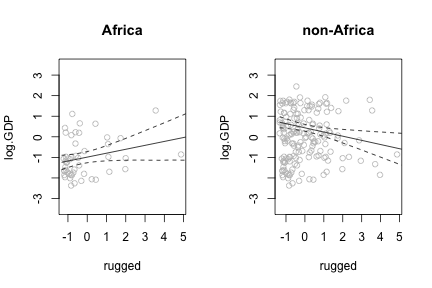
\includegraphics{with-sey} \begin{flushleft}
\ttfamily\noindent
\hlfunctioncall{par}\hlkeyword{(}\hlsymbol{op}\hlkeyword{)}\mbox{}
\normalfont
\end{flushleft}
\end{kframe}}
\end{knitrout}

Model with Seychelles

\begin{knitrout}
\definecolor{shadecolor}{rgb}{.97, .97, .97}{\color{fgcolor}\begin{kframe}
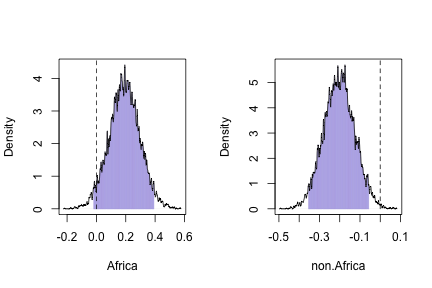
\includegraphics{sey-dens} \end{kframe}}
\end{knitrout}

Posterior densities for effect of ruggedness inside and outside Africa from model {\em with} Seychelles.


\begin{knitrout}
\definecolor{shadecolor}{rgb}{.97, .97, .97}{\color{fgcolor}\begin{kframe}
\begin{flushleft}
\ttfamily\noindent
\hlsymbol{op}{\ }\hlassignement{\usebox{\hlnormalsizeboxlessthan}-}{\ }\hlfunctioncall{par}\hlkeyword{(}\hlargument{mfrow}{\ }\hlargument{=}{\ }\hlfunctioncall{c}\hlkeyword{(}\hlnumber{1}\hlkeyword{,}{\ }\hlnumber{2}\hlkeyword{)}\hlkeyword{)}\hspace*{\fill}\\
\hlstd{}\hlkeyword{for}{\ }\hlkeyword{(}\hlsymbol{AFRICA}{\ }\hlkeyword{in}{\ }\hlfunctioncall{c}\hlkeyword{(}\hlnumber{1}\hlkeyword{,}{\ }\hlnumber{0}\hlkeyword{)}\hlkeyword{)}{\ }\hlkeyword{\usebox{\hlnormalsizeboxopenbrace}}\hspace*{\fill}\\
\hlstd{}{\ }{\ }{\ }{\ }\hlcomment{\usebox{\hlnormalsizeboxhash}\usebox{\hlnormalsizeboxhash}PI{\ }\usebox{\hlnormalsizeboxlessthan}-{\ }sapply(rug.seq,{\ }function(z){\ }PCI(with(post.nS,}\hspace*{\fill}\\
\hlstd{}{\ }{\ }{\ }{\ }\hlcomment{\usebox{\hlnormalsizeboxhash}{\ }{\ }{\ }rnorm(n=NREP,mean=a+a.A*AFRICA+b.r*z+b.Ar*AFRICA*z,sd=sigma))))}\hspace*{\fill}\\
\hlstd{}{\ }{\ }{\ }{\ }\hlsymbol{CI}{\ }\hlassignement{\usebox{\hlnormalsizeboxlessthan}-}{\ }\hlfunctioncall{sapply}\hlkeyword{(}\hlsymbol{rug.seq}\hlkeyword{,}{\ }\hlkeyword{function}\hlkeyword{(}\hlformalargs{z}\hlkeyword{)}{\ }\hlfunctioncall{PCI}\hlkeyword{(}\hlfunctioncall{with}\hlkeyword{(}\hlsymbol{post.nS}\hlkeyword{,}{\ }\hlsymbol{a}{\ }\hlkeyword{+}{\ }\hlsymbol{a.A}{\ }\hlkeyword{*}{\ }\hlsymbol{AFRICA}{\ }\hlkeyword{+}\hspace*{\fill}\\
\hlstd{}{\ }{\ }{\ }{\ }{\ }{\ }{\ }{\ }\hlsymbol{b.r}{\ }\hlkeyword{*}{\ }\hlsymbol{z}{\ }\hlkeyword{+}{\ }\hlsymbol{b.Ar}{\ }\hlkeyword{*}{\ }\hlsymbol{AFRICA}{\ }\hlkeyword{*}{\ }\hlsymbol{z}\hlkeyword{)}\hlkeyword{)}\hlkeyword{)}\hspace*{\fill}\\
\hlstd{}{\ }{\ }{\ }{\ }\hlsymbol{mu}{\ }\hlassignement{\usebox{\hlnormalsizeboxlessthan}-}{\ }\hlfunctioncall{sapply}\hlkeyword{(}\hlsymbol{rug.seq}\hlkeyword{,}{\ }\hlkeyword{function}\hlkeyword{(}\hlformalargs{z}\hlkeyword{)}{\ }\hlfunctioncall{with}\hlkeyword{(}\hlsymbol{mu.coef.nS}\hlkeyword{,}{\ }\hlsymbol{a}{\ }\hlkeyword{+}{\ }\hlsymbol{a.A}{\ }\hlkeyword{*}{\ }\hlsymbol{AFRICA}{\ }\hlkeyword{+}\hspace*{\fill}\\
\hlstd{}{\ }{\ }{\ }{\ }{\ }{\ }{\ }{\ }\hlsymbol{b.r}{\ }\hlkeyword{*}{\ }\hlsymbol{z}{\ }\hlkeyword{+}{\ }\hlsymbol{b.Ar}{\ }\hlkeyword{*}{\ }\hlsymbol{AFRICA}{\ }\hlkeyword{*}{\ }\hlsymbol{z}\hlkeyword{)}\hlkeyword{)}\hspace*{\fill}\\
\hlstd{}\hspace*{\fill}\\
\hlstd{}{\ }{\ }{\ }{\ }\hlfunctioncall{plot}\hlkeyword{(}\hlsymbol{log.GDP}{\ }\hlkeyword{\urltilda{}}{\ }\hlsymbol{rugged}\hlkeyword{,}{\ }\hlargument{data}{\ }\hlargument{=}{\ }\hlsymbol{d.noS}\hlkeyword{[}\hlsymbol{d.rc}\hlkeyword{\usebox{\hlnormalsizeboxdollar}}\hlsymbol{Africa.i}{\ }=={\ }\hlnumber{1}\hlkeyword{,}{\ }\hlkeyword{]}\hlkeyword{,}{\ }\hlargument{ylim}{\ }\hlargument{=}{\ }\hlfunctioncall{c}\hlkeyword{(}\hlkeyword{-}\hlnumber{3.5}\hlkeyword{,}\hspace*{\fill}\\
\hlstd{}{\ }{\ }{\ }{\ }{\ }{\ }{\ }{\ }\hlnumber{3.5}\hlkeyword{)}\hlkeyword{,}{\ }\hlargument{main}{\ }\hlargument{=}{\ }\hlstring{"Africa"}\hlkeyword{,}{\ }\hlargument{col}{\ }\hlargument{=}{\ }\hlfunctioncall{col.alpha}\hlkeyword{(}\hlstring{"gray"}\hlkeyword{,}{\ }\hlnumber{0.9}\hlkeyword{)}\hlkeyword{)}\hspace*{\fill}\\
\hlstd{}{\ }{\ }{\ }{\ }\hlfunctioncall{lines}\hlkeyword{(}\hlsymbol{CI}\hlkeyword{[}\hlnumber{1}\hlkeyword{,}{\ }\hlkeyword{]}{\ }\hlkeyword{\urltilda{}}{\ }\hlsymbol{rug.seq}\hlkeyword{,}{\ }\hlargument{lty}{\ }\hlargument{=}{\ }\hlnumber{2}\hlkeyword{)}\hspace*{\fill}\\
\hlstd{}{\ }{\ }{\ }{\ }\hlfunctioncall{lines}\hlkeyword{(}\hlsymbol{CI}\hlkeyword{[}\hlnumber{2}\hlkeyword{,}{\ }\hlkeyword{]}{\ }\hlkeyword{\urltilda{}}{\ }\hlsymbol{rug.seq}\hlkeyword{,}{\ }\hlargument{lty}{\ }\hlargument{=}{\ }\hlnumber{2}\hlkeyword{)}\hspace*{\fill}\\
\hlstd{}{\ }{\ }{\ }{\ }\hlfunctioncall{lines}\hlkeyword{(}\hlsymbol{mu}{\ }\hlkeyword{\urltilda{}}{\ }\hlsymbol{rug.seq}\hlkeyword{)}\hspace*{\fill}\\
\hlstd{}\hlkeyword{\usebox{\hlnormalsizeboxclosebrace}}\mbox{}
\normalfont
\end{flushleft}
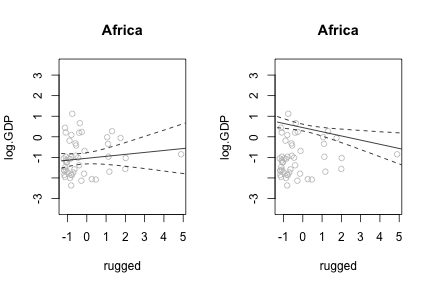
\includegraphics{no-sey} \begin{flushleft}
\ttfamily\noindent
\hlfunctioncall{par}\hlkeyword{(}\hlsymbol{op}\hlkeyword{)}\mbox{}
\normalfont
\end{flushleft}
\end{kframe}}
\end{knitrout}

Model without Seychelles

\begin{knitrout}
\definecolor{shadecolor}{rgb}{.97, .97, .97}{\color{fgcolor}\begin{kframe}
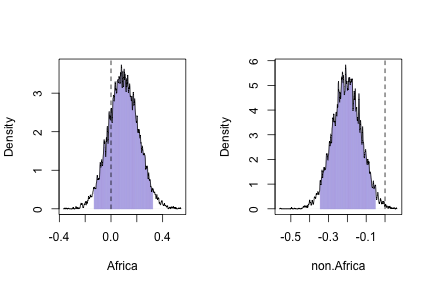
\includegraphics{no-sey-dens} \end{kframe}}
\end{knitrout}

Posterior densities for effect of ruggedness inside and outside Africa from model without Seychelles.

From the plots above, of posterior density and mean effect with confidence intervals both with and without the Seychelles, indicate that the effect of ruggedness {\em does depend on continent}. 
In either case, the effect {\em outside} Africa is strong and negative. 
Within Africa, the effect depends on whether we include Seychelles. With Seychelles, the effect is positive but not strong (0.2, but with CI overlapping with 0). 
Without Seychelles, however, the effect is very weak (0.1, CI strongly overlapping 0).

In either case there is an interaction.

(c) 

\begin{knitrout}
\definecolor{shadecolor}{rgb}{.97, .97, .97}{\color{fgcolor}\begin{kframe}
\begin{flushleft}
\ttfamily\noindent
\hlsymbol{m1}{\ }\hlassignement{\usebox{\hlnormalsizeboxlessthan}-}{\ }\hlfunctioncall{lm.to.mle2}\hlkeyword{(}\hlfunctioncall{lm}\hlkeyword{(}\hlsymbol{log.GDP}{\ }\hlkeyword{\urltilda{}}{\ }\hlsymbol{rugged}\hlkeyword{,}{\ }\hlargument{data}{\ }\hlargument{=}{\ }\hlsymbol{d.rc}\hlkeyword{)}\hlkeyword{,}{\ }\hlargument{data}{\ }\hlargument{=}{\ }\hlsymbol{d.rc}\hlkeyword{)}\hspace*{\fill}\\
\hlstd{}\hlsymbol{m2}{\ }\hlassignement{\usebox{\hlnormalsizeboxlessthan}-}{\ }\hlfunctioncall{lm.to.mle2}\hlkeyword{(}\hlfunctioncall{lm}\hlkeyword{(}\hlsymbol{log.GDP}{\ }\hlkeyword{\urltilda{}}{\ }\hlsymbol{Africa.i}{\ }\hlkeyword{+}{\ }\hlsymbol{rugged}\hlkeyword{,}{\ }\hlargument{data}{\ }\hlargument{=}{\ }\hlsymbol{d.rc}\hlkeyword{)}\hlkeyword{,}\hspace*{\fill}\\
\hlstd{}{\ }{\ }{\ }{\ }\hlargument{data}{\ }\hlargument{=}{\ }\hlsymbol{d.rc}\hlkeyword{)}\hspace*{\fill}\\
\hlstd{}\hlsymbol{m3}{\ }\hlassignement{\usebox{\hlnormalsizeboxlessthan}-}{\ }\hlfunctioncall{lm.to.mle2}\hlkeyword{(}\hlfunctioncall{lm}\hlkeyword{(}\hlsymbol{log.GDP}{\ }\hlkeyword{\urltilda{}}{\ }\hlsymbol{Africa.i}{\ }\hlkeyword{*}{\ }\hlsymbol{rugged}\hlkeyword{,}{\ }\hlargument{data}{\ }\hlargument{=}{\ }\hlsymbol{d.rc}\hlkeyword{)}\hlkeyword{,}\hspace*{\fill}\\
\hlstd{}{\ }{\ }{\ }{\ }\hlargument{data}{\ }\hlargument{=}{\ }\hlsymbol{d.rc}\hlkeyword{)}\hspace*{\fill}\\
\hlstd{}\hspace*{\fill}\\
\hlstd{}\hlsymbol{m1.nS}{\ }\hlassignement{\usebox{\hlnormalsizeboxlessthan}-}{\ }\hlfunctioncall{lm.to.mle2}\hlkeyword{(}\hlfunctioncall{lm}\hlkeyword{(}\hlsymbol{log.GDP}{\ }\hlkeyword{\urltilda{}}{\ }\hlsymbol{rugged}\hlkeyword{,}{\ }\hlargument{data}{\ }\hlargument{=}{\ }\hlsymbol{d.noS}\hlkeyword{)}\hlkeyword{,}{\ }\hlargument{data}{\ }\hlargument{=}{\ }\hlsymbol{d.noS}\hlkeyword{)}\hspace*{\fill}\\
\hlstd{}\hlsymbol{m2.nS}{\ }\hlassignement{\usebox{\hlnormalsizeboxlessthan}-}{\ }\hlfunctioncall{lm.to.mle2}\hlkeyword{(}\hlfunctioncall{lm}\hlkeyword{(}\hlsymbol{log.GDP}{\ }\hlkeyword{\urltilda{}}{\ }\hlsymbol{Africa.i}{\ }\hlkeyword{+}{\ }\hlsymbol{rugged}\hlkeyword{,}{\ }\hlargument{data}{\ }\hlargument{=}{\ }\hlsymbol{d.noS}\hlkeyword{)}\hlkeyword{,}\hspace*{\fill}\\
\hlstd{}{\ }{\ }{\ }{\ }\hlargument{data}{\ }\hlargument{=}{\ }\hlsymbol{d.noS}\hlkeyword{)}\hspace*{\fill}\\
\hlstd{}\hlsymbol{m3.nS}{\ }\hlassignement{\usebox{\hlnormalsizeboxlessthan}-}{\ }\hlfunctioncall{lm.to.mle2}\hlkeyword{(}\hlfunctioncall{lm}\hlkeyword{(}\hlsymbol{log.GDP}{\ }\hlkeyword{\urltilda{}}{\ }\hlsymbol{Africa.i}{\ }\hlkeyword{*}{\ }\hlsymbol{rugged}\hlkeyword{,}{\ }\hlargument{data}{\ }\hlargument{=}{\ }\hlsymbol{d.noS}\hlkeyword{)}\hlkeyword{,}\hspace*{\fill}\\
\hlstd{}{\ }{\ }{\ }{\ }\hlargument{data}{\ }\hlargument{=}{\ }\hlsymbol{d.noS}\hlkeyword{)}\hspace*{\fill}\\
\hlstd{}\hspace*{\fill}\\
\hlstd{}\hlcomment{\usebox{\hlnormalsizeboxhash}with{\ }Seychelles}\hspace*{\fill}\\
\hlstd{}\hlfunctioncall{compare}\hlkeyword{(}\hlsymbol{m1}\hlkeyword{,}{\ }\hlsymbol{m2}\hlkeyword{,}{\ }\hlsymbol{m3}\hlkeyword{,}{\ }\hlargument{nobs}{\ }\hlargument{=}{\ }\hlfunctioncall{nrow}\hlkeyword{(}\hlsymbol{d.rc}\hlkeyword{)}\hlkeyword{)}\mbox{}
\normalfont
\end{flushleft}
\begin{verbatim}
##    k  AICc   BIC    w.AICc     w.BIC  dAICc   dBIC
## m3 5 469.1 484.4   0.96748    0.8684  0.000  0.000
## m2 4 475.9 488.2   0.03252    0.1316  6.786  3.773
## m1 3 539.9 549.2 4.026e-16 7.442e-15 70.831 64.781
\end{verbatim}
\begin{flushleft}
\ttfamily\noindent
\hlcomment{\usebox{\hlnormalsizeboxhash}without{\ }Seychelles}\hspace*{\fill}\\
\hlstd{}\hlfunctioncall{compare}\hlkeyword{(}\hlsymbol{m1.nS}\hlkeyword{,}{\ }\hlsymbol{m2.nS}\hlkeyword{,}{\ }\hlsymbol{m3.nS}\hlkeyword{,}{\ }\hlargument{nobs}{\ }\hlargument{=}{\ }\hlfunctioncall{nrow}\hlkeyword{(}\hlsymbol{d.rc}\hlkeyword{)}\hlkeyword{)}\mbox{}
\normalfont
\end{flushleft}
\begin{verbatim}
##       k  AICc   BIC w.AICc     w.BIC  dAICc    dBIC
## m3.nS 5 463.7 479.0 0.7726    0.4304  0.000  0.5601
## m2.nS 4 466.2 478.5 0.2274    0.5696  2.446  0.0000
## m1.nS 3 536.5 545.8 <2e-16 1.381e-15 72.784 67.3057
\end{verbatim}
\end{kframe}}
\end{knitrout}


\begin{knitrout}
\definecolor{shadecolor}{rgb}{.97, .97, .97}{\color{fgcolor}\begin{kframe}
\begin{flushleft}
\ttfamily\noindent
\hlsymbol{NREP}{\ }\hlassignement{\usebox{\hlnormalsizeboxlessthan}-}{\ }\hlnumber{3e+05}\hspace*{\fill}\\
\hlstd{}\hlsymbol{post.noS}{\ }\hlassignement{\usebox{\hlnormalsizeboxlessthan}-}{\ }\hlfunctioncall{sample.naive.posterior}\hlkeyword{(}\hlfunctioncall{list}\hlkeyword{(}\hlsymbol{m1.nS}\hlkeyword{,}{\ }\hlsymbol{m2.nS}\hlkeyword{,}{\ }\hlsymbol{m3.nS}\hlkeyword{)}\hlkeyword{,}\hspace*{\fill}\\
\hlstd{}{\ }{\ }{\ }{\ }\hlargument{n}{\ }\hlargument{=}{\ }\hlsymbol{NREP}\hlkeyword{,}{\ }\hlargument{method}{\ }\hlargument{=}{\ }\hlstring{"AICc"}\hlkeyword{,}{\ }\hlargument{nobs}{\ }\hlargument{=}{\ }\hlfunctioncall{nrow}\hlkeyword{(}\hlsymbol{d.noS}\hlkeyword{)}\hlkeyword{)}\mbox{}
\normalfont
\end{flushleft}
\begin{verbatim}
## Warning message: One or more models produced zero samples, because of very low posterior probability.
\end{verbatim}
\begin{flushleft}
\ttfamily\noindent
\hspace*{\fill}\\
\hlstd{}\hlsymbol{mu.coef}{\ }\hlassignement{\usebox{\hlnormalsizeboxlessthan}-}{\ }\hlfunctioncall{as.list}\hlkeyword{(}\hlfunctioncall{colMeans}\hlkeyword{(}\hlsymbol{post.noS}\hlkeyword{)}\hlkeyword{)}\hspace*{\fill}\\
\hlstd{}\hlsymbol{rug.seq}{\ }\hlassignement{\usebox{\hlnormalsizeboxlessthan}-}{\ }\hlfunctioncall{with}\hlkeyword{(}\hlsymbol{d.noS}\hlkeyword{,}{\ }\hlfunctioncall{seq}\hlkeyword{(}\hlfunctioncall{min}\hlkeyword{(}\hlsymbol{rugged}\hlkeyword{)}\hlkeyword{,}{\ }\hlfunctioncall{max}\hlkeyword{(}\hlsymbol{rugged}\hlkeyword{)}{\ }\hlkeyword{+}{\ }\hlnumber{2}\hlkeyword{,}\hspace*{\fill}\\
\hlstd{}{\ }{\ }{\ }{\ }\hlargument{length.out}{\ }\hlargument{=}{\ }\hlnumber{100}\hlkeyword{)}\hlkeyword{)}\mbox{}
\normalfont
\end{flushleft}
\end{kframe}}
\end{knitrout}


\begin{knitrout}
\definecolor{shadecolor}{rgb}{.97, .97, .97}{\color{fgcolor}\begin{kframe}
\begin{flushleft}
\ttfamily\noindent
\hlsymbol{op}{\ }\hlassignement{\usebox{\hlnormalsizeboxlessthan}-}{\ }\hlfunctioncall{par}\hlkeyword{(}\hlargument{mfrow}{\ }\hlargument{=}{\ }\hlfunctioncall{c}\hlkeyword{(}\hlnumber{1}\hlkeyword{,}{\ }\hlnumber{2}\hlkeyword{)}\hlkeyword{)}\hspace*{\fill}\\
\hlstd{}\hlkeyword{for}{\ }\hlkeyword{(}\hlsymbol{AFRICA}{\ }\hlkeyword{in}{\ }\hlfunctioncall{c}\hlkeyword{(}\hlnumber{1}\hlkeyword{,}{\ }\hlnumber{0}\hlkeyword{)}\hlkeyword{)}{\ }\hlkeyword{\usebox{\hlnormalsizeboxopenbrace}}\hspace*{\fill}\\
\hlstd{}{\ }{\ }{\ }{\ }\hlsymbol{PI}{\ }\hlassignement{\usebox{\hlnormalsizeboxlessthan}-}{\ }\hlfunctioncall{sapply}\hlkeyword{(}\hlsymbol{rug.seq}\hlkeyword{,}{\ }\hlkeyword{function}\hlkeyword{(}\hlformalargs{z}\hlkeyword{)}{\ }\hlfunctioncall{PCI}\hlkeyword{(}\hlfunctioncall{with}\hlkeyword{(}\hlsymbol{post.noS}\hlkeyword{,}{\ }\hlfunctioncall{rnorm}\hlkeyword{(}\hlargument{n}{\ }\hlargument{=}{\ }\hlsymbol{NREP}\hlkeyword{,}\hspace*{\fill}\\
\hlstd{}{\ }{\ }{\ }{\ }{\ }{\ }{\ }{\ }\hlargument{mean}{\ }\hlargument{=}{\ }\hlsymbol{a}{\ }\hlkeyword{+}{\ }\hlsymbol{b1}{\ }\hlkeyword{*}{\ }\hlsymbol{AFRICA}{\ }\hlkeyword{+}{\ }\hlsymbol{b2}{\ }\hlkeyword{*}{\ }\hlsymbol{z}{\ }\hlkeyword{+}{\ }\hlsymbol{b3}{\ }\hlkeyword{*}{\ }\hlsymbol{AFRICA}{\ }\hlkeyword{*}{\ }\hlsymbol{z}\hlkeyword{,}{\ }\hlargument{sd}{\ }\hlargument{=}{\ }\hlnumber{1}\hlkeyword{/}\hlsymbol{tau}\hlkeyword{)}\hlkeyword{)}\hlkeyword{)}\hlkeyword{)}\hspace*{\fill}\\
\hlstd{}{\ }{\ }{\ }{\ }\hlsymbol{CI}{\ }\hlassignement{\usebox{\hlnormalsizeboxlessthan}-}{\ }\hlfunctioncall{sapply}\hlkeyword{(}\hlsymbol{rug.seq}\hlkeyword{,}{\ }\hlkeyword{function}\hlkeyword{(}\hlformalargs{z}\hlkeyword{)}{\ }\hlfunctioncall{PCI}\hlkeyword{(}\hlfunctioncall{with}\hlkeyword{(}\hlsymbol{post.noS}\hlkeyword{,}{\ }\hlsymbol{a}{\ }\hlkeyword{+}{\ }\hlsymbol{b1}{\ }\hlkeyword{*}{\ }\hlsymbol{AFRICA}{\ }\hlkeyword{+}\hspace*{\fill}\\
\hlstd{}{\ }{\ }{\ }{\ }{\ }{\ }{\ }{\ }\hlsymbol{b2}{\ }\hlkeyword{*}{\ }\hlsymbol{z}{\ }\hlkeyword{+}{\ }\hlsymbol{b3}{\ }\hlkeyword{*}{\ }\hlsymbol{AFRICA}{\ }\hlkeyword{*}{\ }\hlsymbol{z}\hlkeyword{)}\hlkeyword{)}\hlkeyword{)}\hspace*{\fill}\\
\hlstd{}{\ }{\ }{\ }{\ }\hlsymbol{mu}{\ }\hlassignement{\usebox{\hlnormalsizeboxlessthan}-}{\ }\hlfunctioncall{sapply}\hlkeyword{(}\hlsymbol{rug.seq}\hlkeyword{,}{\ }\hlkeyword{function}\hlkeyword{(}\hlformalargs{z}\hlkeyword{)}{\ }\hlfunctioncall{with}\hlkeyword{(}\hlsymbol{mu.coef}\hlkeyword{,}{\ }\hlsymbol{a}{\ }\hlkeyword{+}{\ }\hlsymbol{b1}{\ }\hlkeyword{*}{\ }\hlsymbol{AFRICA}{\ }\hlkeyword{+}\hspace*{\fill}\\
\hlstd{}{\ }{\ }{\ }{\ }{\ }{\ }{\ }{\ }\hlsymbol{b2}{\ }\hlkeyword{*}{\ }\hlsymbol{z}{\ }\hlkeyword{+}{\ }\hlsymbol{b3}{\ }\hlkeyword{*}{\ }\hlsymbol{AFRICA}{\ }\hlkeyword{*}{\ }\hlsymbol{z}\hlkeyword{)}\hlkeyword{)}\hspace*{\fill}\\
\hlstd{}{\ }{\ }{\ }{\ }\hlfunctioncall{plot}\hlkeyword{(}\hlsymbol{log.GDP}{\ }\hlkeyword{\urltilda{}}{\ }\hlsymbol{rugged}\hlkeyword{,}{\ }\hlargument{data}{\ }\hlargument{=}{\ }\hlsymbol{d.noS}\hlkeyword{[}\hlsymbol{d.noS}\hlkeyword{\usebox{\hlnormalsizeboxdollar}}\hlsymbol{Africa.i}{\ }=={\ }\hlnumber{1}\hlkeyword{,}{\ }\hlkeyword{]}\hlkeyword{,}{\ }\hlargument{ylim}{\ }\hlargument{=}{\ }\hlfunctioncall{c}\hlkeyword{(}\hlkeyword{-}\hlnumber{3.5}\hlkeyword{,}\hspace*{\fill}\\
\hlstd{}{\ }{\ }{\ }{\ }{\ }{\ }{\ }{\ }\hlnumber{3.5}\hlkeyword{)}\hlkeyword{,}{\ }\hlargument{main}{\ }\hlargument{=}{\ }\hlstring{"Africa"}\hlkeyword{,}{\ }\hlargument{col}{\ }\hlargument{=}{\ }\hlfunctioncall{col.alpha}\hlkeyword{(}\hlstring{"gray"}\hlkeyword{,}{\ }\hlnumber{0.9}\hlkeyword{)}\hlkeyword{)}\hspace*{\fill}\\
\hlstd{}{\ }{\ }{\ }{\ }\hlfunctioncall{lines}\hlkeyword{(}\hlsymbol{CI}\hlkeyword{[}\hlnumber{1}\hlkeyword{,}{\ }\hlkeyword{]}{\ }\hlkeyword{\urltilda{}}{\ }\hlsymbol{rug.seq}\hlkeyword{,}{\ }\hlargument{lty}{\ }\hlargument{=}{\ }\hlnumber{2}\hlkeyword{)}\hspace*{\fill}\\
\hlstd{}{\ }{\ }{\ }{\ }\hlfunctioncall{lines}\hlkeyword{(}\hlsymbol{CI}\hlkeyword{[}\hlnumber{2}\hlkeyword{,}{\ }\hlkeyword{]}{\ }\hlkeyword{\urltilda{}}{\ }\hlsymbol{rug.seq}\hlkeyword{,}{\ }\hlargument{lty}{\ }\hlargument{=}{\ }\hlnumber{2}\hlkeyword{)}\hspace*{\fill}\\
\hlstd{}{\ }{\ }{\ }{\ }\hlfunctioncall{lines}\hlkeyword{(}\hlsymbol{PI}\hlkeyword{[}\hlnumber{1}\hlkeyword{,}{\ }\hlkeyword{]}{\ }\hlkeyword{\urltilda{}}{\ }\hlsymbol{rug.seq}\hlkeyword{,}{\ }\hlargument{lty}{\ }\hlargument{=}{\ }\hlnumber{3}\hlkeyword{)}\hspace*{\fill}\\
\hlstd{}{\ }{\ }{\ }{\ }\hlfunctioncall{lines}\hlkeyword{(}\hlsymbol{PI}\hlkeyword{[}\hlnumber{2}\hlkeyword{,}{\ }\hlkeyword{]}{\ }\hlkeyword{\urltilda{}}{\ }\hlsymbol{rug.seq}\hlkeyword{,}{\ }\hlargument{lty}{\ }\hlargument{=}{\ }\hlnumber{3}\hlkeyword{)}\hspace*{\fill}\\
\hlstd{}{\ }{\ }{\ }{\ }\hlfunctioncall{lines}\hlkeyword{(}\hlsymbol{mu}{\ }\hlkeyword{\urltilda{}}{\ }\hlsymbol{rug.seq}\hlkeyword{)}\hspace*{\fill}\\
\hlstd{}\hlkeyword{\usebox{\hlnormalsizeboxclosebrace}}\mbox{}
\normalfont
\end{flushleft}
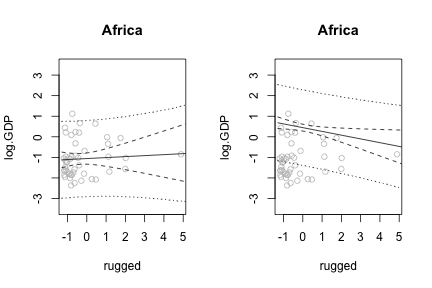
\includegraphics{AICc-avg} \begin{flushleft}
\ttfamily\noindent
\hlfunctioncall{par}\hlkeyword{(}\hlsymbol{op}\hlkeyword{)}\mbox{}
\normalfont
\end{flushleft}
\end{kframe}}
\end{knitrout}

Fits to data without Seychelles for averaged model (based on AICc), as well as confidence intervals for the mean and prediction intervals.

The predictions of the averaged model agree with the above inferences, but provide stronger support for no effect of ruggedness within Africa. 
The effect of ruggedness does, however, change with continent. 
In all cases, I infer an interaction.

\begin{knitrout}
\definecolor{shadecolor}{rgb}{.97, .97, .97}{\color{fgcolor}\begin{kframe}
\begin{flushleft}
\ttfamily\noindent
\hspace*{\fill}\\
\hlstd{}\hlsymbol{\usebox{\hlnormalsizeboxbacktick}non-Africa\usebox{\hlnormalsizeboxbacktick}}{\ }\hlassignement{\usebox{\hlnormalsizeboxlessthan}-}{\ }\hlsymbol{post.noS}\hlkeyword{\usebox{\hlnormalsizeboxdollar}}\hlsymbol{b2}{\ }\hlkeyword{+}{\ }\hlsymbol{post.noS}\hlkeyword{\usebox{\hlnormalsizeboxdollar}}\hlsymbol{b3}{\ }\hlkeyword{*}{\ }\hlnumber{0}\hspace*{\fill}\\
\hlstd{}\hlsymbol{Africa}{\ }\hlassignement{\usebox{\hlnormalsizeboxlessthan}-}{\ }\hlsymbol{post.noS}\hlkeyword{\usebox{\hlnormalsizeboxdollar}}\hlsymbol{b2}{\ }\hlkeyword{+}{\ }\hlsymbol{post.noS}\hlkeyword{\usebox{\hlnormalsizeboxdollar}}\hlsymbol{b3}{\ }\hlkeyword{*}{\ }\hlnumber{1}\hspace*{\fill}\\
\hlstd{}\hlfunctioncall{dens}\hlkeyword{(}\hlfunctioncall{data.frame}\hlkeyword{(}\hlsymbol{Africa}\hlkeyword{,}{\ }\hlsymbol{\usebox{\hlnormalsizeboxbacktick}non-Africa\usebox{\hlnormalsizeboxbacktick}}\hlkeyword{)}\hlkeyword{)}\mbox{}
\normalfont
\end{flushleft}
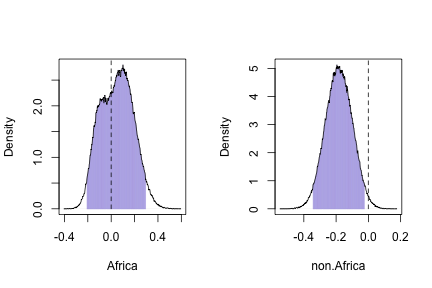
\includegraphics{AICc-dens} \end{kframe}}
\end{knitrout}

Posterior densities for effect of ruggedness inside and outside Africa from average model (AICc) without Seychelles.

\subsection*{Language diversity }


We want to evaluate the hypothesis that language diversity is related to food security. 
In particular, the causal idea is that productive land and climate lead to smaller ethnic groups, as there is less need for trade.

For this task, we use data from Nettle (1998): 

\begin{knitrout}
\definecolor{shadecolor}{rgb}{.97, .97, .97}{\color{fgcolor}\begin{kframe}
\begin{flushleft}
\ttfamily\noindent
\hlfunctioncall{data}\hlkeyword{(}\hlsymbol{nettle}\hlkeyword{)}\hspace*{\fill}\\
\hlstd{}\hlfunctioncall{head}\hlkeyword{(}\hlsymbol{nettle}\hlkeyword{,}{\ }\hlargument{n}{\ }\hlargument{=}{\ }\hlnumber{1}\hlkeyword{)}\mbox{}
\normalfont
\end{flushleft}
\begin{verbatim}
##   country num.lang    area k.pop num.stations mean.growing.season sd.growing.season
## 1 Algeria       18 2381741 25660          102                 6.6              2.29
\end{verbatim}
\begin{flushleft}
\ttfamily\noindent
\hlsymbol{d}{\ }\hlassignement{\usebox{\hlnormalsizeboxlessthan}-}{\ }\hlsymbol{nettle}\hspace*{\fill}\\
\hlstd{}\hlsymbol{d}\hlkeyword{\usebox{\hlnormalsizeboxdollar}}\hlsymbol{lang.per.cap}{\ }\hlassignement{\usebox{\hlnormalsizeboxlessthan}-}{\ }\hlsymbol{d}\hlkeyword{\usebox{\hlnormalsizeboxdollar}}\hlsymbol{num.lang}\hlkeyword{/}\hlsymbol{d}\hlkeyword{\usebox{\hlnormalsizeboxdollar}}\hlsymbol{k.pop}\hspace*{\fill}\\
\hlstd{}\hlsymbol{d}\hlkeyword{\usebox{\hlnormalsizeboxdollar}}\hlsymbol{log.lpc}{\ }\hlassignement{\usebox{\hlnormalsizeboxlessthan}-}{\ }\hlfunctioncall{log}\hlkeyword{(}\hlsymbol{d}\hlkeyword{\usebox{\hlnormalsizeboxdollar}}\hlsymbol{lang.per.cap}\hlkeyword{)}\mbox{}
\normalfont
\end{flushleft}
\end{kframe}}
\end{knitrout}


No pair-wise correlations are super high: 
\begin{knitrout}
\definecolor{shadecolor}{rgb}{.97, .97, .97}{\color{fgcolor}\begin{kframe}
\begin{flushleft}
\ttfamily\noindent
\hlfunctioncall{cor}\hlkeyword{(}\hlsymbol{d}\hlkeyword{[}\hlkeyword{,}{\ }\hlfunctioncall{c}\hlkeyword{(}\hlstring{"log.lpc"}\hlkeyword{,}{\ }\hlstring{"area"}\hlkeyword{,}{\ }\hlstring{"mean.growing.season"}\hlkeyword{,}{\ }\hlstring{"sd.growing.season"}\hlkeyword{)}\hlkeyword{]}\hlkeyword{)}\mbox{}
\normalfont
\end{flushleft}
\begin{verbatim}
##                     log.lpc    area mean.growing.season sd.growing.season
## log.lpc              1.0000 -0.1375             0.35964          -0.25339
## area                -0.1375  1.0000            -0.12898           0.60452
## mean.growing.season  0.3596 -0.1290             1.00000           0.02136
## sd.growing.season   -0.2534  0.6045             0.02136           1.00000
\end{verbatim}
\begin{flushleft}
\ttfamily\noindent
\hlsymbol{d.rc}{\ }\hlassignement{\usebox{\hlnormalsizeboxlessthan}-}{\ }\hlsymbol{d}\hspace*{\fill}\\
\hlstd{}\hlsymbol{d.rc}\hlkeyword{[}\hlkeyword{,}{\ }\hlfunctioncall{c}\hlkeyword{(}\hlstring{"mean.growing.season"}\hlkeyword{,}{\ }\hlstring{"sd.growing.season"}\hlkeyword{)}\hlkeyword{]}{\ }\hlassignement{\usebox{\hlnormalsizeboxlessthan}-}{\ }\hlfunctioncall{apply}\hlkeyword{(}\hlsymbol{d.rc}\hlkeyword{[}\hlkeyword{,}\hspace*{\fill}\\
\hlstd{}{\ }{\ }{\ }{\ }\hlfunctioncall{c}\hlkeyword{(}\hlstring{"mean.growing.season"}\hlkeyword{,}{\ }\hlstring{"sd.growing.season"}\hlkeyword{)}\hlkeyword{]}\hlkeyword{,}{\ }\hlnumber{2}\hlkeyword{,}{\ }\hlkeyword{function}\hlkeyword{(}\hlformalargs{x}\hlkeyword{)}{\ }\hlsymbol{x}{\ }\hlkeyword{-}\hspace*{\fill}\\
\hlstd{}{\ }{\ }{\ }{\ }\hlfunctioncall{mean}\hlkeyword{(}\hlsymbol{x}\hlkeyword{)}\hlkeyword{)}\mbox{}
\normalfont
\end{flushleft}
\end{kframe}}
\end{knitrout}


Evaluate the models using mean and standard deviation, their interaction, and logarithm of area as predictors of the log languages per captia: 

(a,b,c)

\begin{knitrout}
\definecolor{shadecolor}{rgb}{.97, .97, .97}{\color{fgcolor}\begin{kframe}
\begin{flushleft}
\ttfamily\noindent
\hlsymbol{m1}{\ }\hlassignement{\usebox{\hlnormalsizeboxlessthan}-}{\ }\hlfunctioncall{lm}\hlkeyword{(}\hlfunctioncall{log}\hlkeyword{(}\hlsymbol{lang.per.cap}\hlkeyword{)}{\ }\hlkeyword{\urltilda{}}{\ }\hlsymbol{mean.growing.season}{\ }\hlkeyword{+}{\ }\hlfunctioncall{log}\hlkeyword{(}\hlsymbol{area}\hlkeyword{)}\hlkeyword{,}\hspace*{\fill}\\
\hlstd{}{\ }{\ }{\ }{\ }\hlargument{data}{\ }\hlargument{=}{\ }\hlsymbol{d.rc}\hlkeyword{)}\hspace*{\fill}\\
\hlstd{}\hlfunctioncall{precis}\hlkeyword{(}\hlsymbol{m1}\hlkeyword{)}\mbox{}
\normalfont
\end{flushleft}
\begin{verbatim}
##                     Estimate Std. Error     2.5%   97.5%
## (Intercept)          -2.8469    1.82311 -6.42010 0.72635
## mean.growing.season   0.1438    0.05682  0.03245 0.25517
## log(area)            -0.2018    0.14037 -0.47687 0.07336
\end{verbatim}
\begin{flushleft}
\ttfamily\noindent
\hlsymbol{m2}{\ }\hlassignement{\usebox{\hlnormalsizeboxlessthan}-}{\ }\hlfunctioncall{lm}\hlkeyword{(}\hlfunctioncall{log}\hlkeyword{(}\hlsymbol{lang.per.cap}\hlkeyword{)}{\ }\hlkeyword{\urltilda{}}{\ }\hlsymbol{sd.growing.season}{\ }\hlkeyword{+}{\ }\hlfunctioncall{log}\hlkeyword{(}\hlsymbol{area}\hlkeyword{)}\hlkeyword{,}\hspace*{\fill}\\
\hlstd{}{\ }{\ }{\ }{\ }\hlargument{data}{\ }\hlargument{=}{\ }\hlsymbol{d.rc}\hlkeyword{)}\hspace*{\fill}\\
\hlstd{}\hlfunctioncall{precis}\hlkeyword{(}\hlsymbol{m2}\hlkeyword{)}\mbox{}
\normalfont
\end{flushleft}
\begin{verbatim}
##                   Estimate Std. Error    2.5%   97.5%
## (Intercept)        -2.3565     2.0703 -6.4142 1.70126
## sd.growing.season  -0.2093     0.1904 -0.5824 0.16394
## log(area)          -0.2397     0.1595 -0.5523 0.07296
\end{verbatim}
\begin{flushleft}
\ttfamily\noindent
\hlsymbol{m3}{\ }\hlassignement{\usebox{\hlnormalsizeboxlessthan}-}{\ }\hlfunctioncall{lm}\hlkeyword{(}\hlfunctioncall{log}\hlkeyword{(}\hlsymbol{lang.per.cap}\hlkeyword{)}{\ }\hlkeyword{\urltilda{}}{\ }\hlsymbol{mean.growing.season}{\ }\hlkeyword{*}{\ }\hlsymbol{sd.growing.season}\hlkeyword{,}\hspace*{\fill}\\
\hlstd{}{\ }{\ }{\ }{\ }\hlargument{data}{\ }\hlargument{=}{\ }\hlsymbol{d.rc}\hlkeyword{)}\hspace*{\fill}\\
\hlstd{}\hlfunctioncall{precis}\hlkeyword{(}\hlsymbol{m3}\hlkeyword{)}\mbox{}
\normalfont
\end{flushleft}
\begin{verbatim}
##                                       Estimate Std. Error      2.5%    97.5%
## (Intercept)                            -5.4489    0.15621 -5.755087 -5.14275
## mean.growing.season                     0.1147    0.05711  0.002741  0.22662
## sd.growing.season                      -0.3443    0.14806 -0.634518 -0.05412
## mean.growing.season:sd.growing.season  -0.1089    0.04839 -0.203717 -0.01401
\end{verbatim}
\begin{flushleft}
\ttfamily\noindent
\hlsymbol{m4}{\ }\hlassignement{\usebox{\hlnormalsizeboxlessthan}-}{\ }\hlfunctioncall{lm}\hlkeyword{(}\hlfunctioncall{log}\hlkeyword{(}\hlsymbol{lang.per.cap}\hlkeyword{)}{\ }\hlkeyword{\urltilda{}}{\ }\hlsymbol{mean.growing.season}{\ }\hlkeyword{*}{\ }\hlsymbol{sd.growing.season}{\ }\hlkeyword{+}\hspace*{\fill}\\
\hlstd{}{\ }{\ }{\ }{\ }\hlfunctioncall{log}\hlkeyword{(}\hlsymbol{area}\hlkeyword{)}\hlkeyword{,}{\ }\hlargument{data}{\ }\hlargument{=}{\ }\hlsymbol{d.rc}\hlkeyword{)}\hspace*{\fill}\\
\hlstd{}\hlfunctioncall{precis}\hlkeyword{(}\hlsymbol{m4}\hlkeyword{)}\mbox{}
\normalfont
\end{flushleft}
\begin{verbatim}
##                                        Estimate Std. Error     2.5%    97.5%
## (Intercept)                           -5.379279    2.13431 -9.56245 -1.19611
## mean.growing.season                    0.113862    0.06273 -0.00908  0.23680
## sd.growing.season                     -0.340855    0.18293 -0.69939  0.01768
## log(area)                             -0.005384    0.16456 -0.32791  0.31714
## mean.growing.season:sd.growing.season -0.108845    0.04875 -0.20439 -0.01330
\end{verbatim}
\end{kframe}}
\end{knitrout}


After controlling for log area, mean growing season has a positive effect on diversity (m1), while standard deviation in growing season has a weak negative effect (m2). 
When the main effects of mean and variance of growing season as well as their interaction are consided (m3), we find a negative relationship between language diversity and the standard deviation of growing season, but a positive relationship with the mean growing season, as well as  a negative interaction between the standard deviation and mean of growing season. 

Model selection with AICc and BIC indicates little support for using log(area) as a predictor when considering the interaction (m3 v m4).
\begin{knitrout}
\definecolor{shadecolor}{rgb}{.97, .97, .97}{\color{fgcolor}\begin{kframe}
\begin{flushleft}
\ttfamily\noindent
\hlfunctioncall{compare}\hlkeyword{(}\hlsymbol{m3}\hlkeyword{,}{\ }\hlsymbol{m4}\hlkeyword{,}{\ }\hlargument{nobs}{\ }\hlargument{=}{\ }\hlfunctioncall{nrow}\hlkeyword{(}\hlsymbol{d.rc}\hlkeyword{)}\hlkeyword{)}\mbox{}
\normalfont
\end{flushleft}
\begin{verbatim}
##    k  AICc   BIC w.AICc  w.BIC dAICc  dBIC
## m3 5 260.5 271.1 0.7659 0.8958  0.00 0.000
## m4 6 262.8 275.4 0.2341 0.1042  2.37 4.303
\end{verbatim}
\end{kframe}}
\end{knitrout}


The model with the interaction had strong support under both AICc and BIC.  
\begin{knitrout}
\definecolor{shadecolor}{rgb}{.97, .97, .97}{\color{fgcolor}\begin{kframe}
\begin{flushleft}
\ttfamily\noindent
\hlfunctioncall{compare}\hlkeyword{(}\hlsymbol{m1}\hlkeyword{,}{\ }\hlsymbol{m2}\hlkeyword{,}{\ }\hlsymbol{m3}\hlkeyword{,}{\ }\hlargument{nobs}{\ }\hlargument{=}{\ }\hlfunctioncall{nrow}\hlkeyword{(}\hlsymbol{d.rc}\hlkeyword{)}\hlkeyword{)}\mbox{}
\normalfont
\end{flushleft}
\begin{verbatim}
##    k  AICc   BIC  w.AICc    w.BIC  dAICc  dBIC
## m3 5 260.5 271.1 0.96490 0.909965  0.000 0.000
## m1 4 267.2 275.9 0.03261 0.083648  6.775 4.774
## m2 4 272.4 281.0 0.00249 0.006387 11.920 9.918
\end{verbatim}
\end{kframe}}
\end{knitrout}


To better understand the strength of the interaction in determining the relationship between language diversity and growing season, I picked out below average, average, and above average values of the standard deviation and mean. 

\begin{knitrout}
\definecolor{shadecolor}{rgb}{.97, .97, .97}{\color{fgcolor}\begin{kframe}
\begin{flushleft}
\ttfamily\noindent
\hlsymbol{op}{\ }\hlassignement{\usebox{\hlnormalsizeboxlessthan}-}{\ }\hlfunctioncall{par}\hlkeyword{(}\hlargument{mfrow}{\ }\hlargument{=}{\ }\hlfunctioncall{c}\hlkeyword{(}\hlnumber{1}\hlkeyword{,}{\ }\hlnumber{2}\hlkeyword{)}\hlkeyword{)}\hspace*{\fill}\\
\hlstd{}\hlfunctioncall{with}\hlkeyword{(}\hlsymbol{d.rc}\hlkeyword{,}{\ }\hlfunctioncall{hist}\hlkeyword{(}\hlsymbol{mean.growing.season}\hlkeyword{,}{\ }\hlargument{main}{\ }\hlargument{=}{\ }\hlstring{""}\hlkeyword{)}\hlkeyword{)}\hspace*{\fill}\\
\hlstd{}\hlfunctioncall{with}\hlkeyword{(}\hlsymbol{d.rc}\hlkeyword{,}{\ }\hlfunctioncall{hist}\hlkeyword{(}\hlsymbol{sd.growing.season}\hlkeyword{,}{\ }\hlargument{main}{\ }\hlargument{=}{\ }\hlstring{""}\hlkeyword{)}\hlkeyword{)}\mbox{}
\normalfont
\end{flushleft}
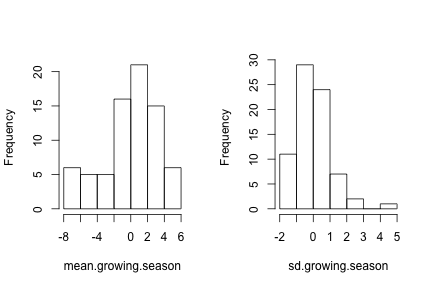
\includegraphics{sd-mean-dist} \begin{flushleft}
\ttfamily\noindent
\hlfunctioncall{par}\hlkeyword{(}\hlsymbol{op}\hlkeyword{)}\mbox{}
\normalfont
\end{flushleft}
\end{kframe}}
\end{knitrout}


These values, based on histograms of the summary statistics, were {\tt sd = -1.5, 0, 1.5} and {\tt mean = -4, 0, 4}. 
For these values, I plotted the effect of the other predictor on mean prediction for model 3. 

(I was interested to average the models, but including area had a strange effect on output. I wasn't sure that averaging over the coefficients was having the intended effect... )

\begin{knitrout}
\definecolor{shadecolor}{rgb}{.97, .97, .97}{\color{fgcolor}\begin{kframe}
\begin{flushleft}
\ttfamily\noindent
\hlsymbol{NREP}{\ }\hlassignement{\usebox{\hlnormalsizeboxlessthan}-}{\ }\hlnumber{3e+05}\hspace*{\fill}\\
\hlstd{}\hlsymbol{post}{\ }\hlassignement{\usebox{\hlnormalsizeboxlessthan}-}{\ }\hlfunctioncall{sample.naive.posterior}\hlkeyword{(}\hlsymbol{m3}\hlkeyword{,}{\ }\hlargument{n}{\ }\hlargument{=}{\ }\hlsymbol{NREP}\hlkeyword{)}{\ }{\ }\hlcomment{\usebox{\hlnormalsizeboxhash},{\ }method=\usebox{\hlnormalsizeboxsinglequote}AICc\usebox{\hlnormalsizeboxsinglequote},{\ }nobs=nrow(d.rc))}\hspace*{\fill}\\
\hlstd{}\hlfunctioncall{names}\hlkeyword{(}\hlsymbol{post}\hlkeyword{)}{\ }\hlassignement{\usebox{\hlnormalsizeboxlessthan}-}{\ }\hlfunctioncall{c}\hlkeyword{(}\hlstring{"a"}\hlkeyword{,}{\ }\hlstring{"b.mu.gs"}\hlkeyword{,}{\ }\hlstring{"b.sd.gs"}\hlkeyword{,}{\ }\hlstring{"b.mu.sd"}\hlkeyword{)}\hspace*{\fill}\\
\hlstd{}\hspace*{\fill}\\
\hlstd{}\hlsymbol{mu.coef}{\ }\hlassignement{\usebox{\hlnormalsizeboxlessthan}-}{\ }\hlfunctioncall{as.list}\hlkeyword{(}\hlfunctioncall{colMeans}\hlkeyword{(}\hlsymbol{post}\hlkeyword{)}\hlkeyword{)}\hspace*{\fill}\\
\hlstd{}\hlsymbol{mean.seq}{\ }\hlassignement{\usebox{\hlnormalsizeboxlessthan}-}{\ }\hlfunctioncall{with}\hlkeyword{(}\hlsymbol{d.rc}\hlkeyword{,}{\ }\hlfunctioncall{seq}\hlkeyword{(}\hlfunctioncall{min}\hlkeyword{(}\hlsymbol{mean.growing.season}\hlkeyword{)}\hlkeyword{,}{\ }\hlfunctioncall{max}\hlkeyword{(}\hlsymbol{mean.growing.season}\hlkeyword{)}{\ }\hlkeyword{+}\hspace*{\fill}\\
\hlstd{}{\ }{\ }{\ }{\ }\hlnumber{1}\hlkeyword{,}{\ }\hlargument{length.out}{\ }\hlargument{=}{\ }\hlnumber{100}\hlkeyword{)}\hlkeyword{)}\hspace*{\fill}\\
\hlstd{}\hlsymbol{sd.seq}{\ }\hlassignement{\usebox{\hlnormalsizeboxlessthan}-}{\ }\hlfunctioncall{with}\hlkeyword{(}\hlsymbol{d.rc}\hlkeyword{,}{\ }\hlfunctioncall{seq}\hlkeyword{(}\hlfunctioncall{min}\hlkeyword{(}\hlsymbol{sd.growing.season}\hlkeyword{)}\hlkeyword{,}{\ }\hlfunctioncall{max}\hlkeyword{(}\hlsymbol{sd.growing.season}\hlkeyword{)}{\ }\hlkeyword{+}\hspace*{\fill}\\
\hlstd{}{\ }{\ }{\ }{\ }\hlnumber{1}\hlkeyword{,}{\ }\hlargument{length.out}{\ }\hlargument{=}{\ }\hlnumber{100}\hlkeyword{)}\hlkeyword{)}\hspace*{\fill}\\
\hlstd{}\hspace*{\fill}\\
\hlstd{}\hlsymbol{op}{\ }\hlassignement{\usebox{\hlnormalsizeboxlessthan}-}{\ }\hlfunctioncall{par}\hlkeyword{(}\hlargument{mfrow}{\ }\hlargument{=}{\ }\hlfunctioncall{c}\hlkeyword{(}\hlnumber{2}\hlkeyword{,}{\ }\hlnumber{3}\hlkeyword{)}\hlkeyword{)}\hspace*{\fill}\\
\hlstd{}\hlkeyword{for}{\ }\hlkeyword{(}\hlsymbol{SD.gs}{\ }\hlkeyword{in}{\ }\hlfunctioncall{c}\hlkeyword{(}\hlkeyword{-}\hlnumber{1.5}\hlkeyword{,}{\ }\hlnumber{0}\hlkeyword{,}{\ }\hlnumber{1.5}\hlkeyword{)}\hlkeyword{)}{\ }\hlkeyword{\usebox{\hlnormalsizeboxopenbrace}}\hspace*{\fill}\\
\hlstd{}{\ }{\ }{\ }{\ }\hlsymbol{CI}{\ }\hlassignement{\usebox{\hlnormalsizeboxlessthan}-}{\ }\hlfunctioncall{sapply}\hlkeyword{(}\hlsymbol{mean.seq}\hlkeyword{,}{\ }\hlkeyword{function}\hlkeyword{(}\hlformalargs{z}\hlkeyword{)}{\ }\hlfunctioncall{PCI}\hlkeyword{(}\hlfunctioncall{with}\hlkeyword{(}\hlsymbol{post}\hlkeyword{,}{\ }\hlsymbol{a}{\ }\hlkeyword{+}{\ }\hlsymbol{b.mu.gs}{\ }\hlkeyword{*}\hspace*{\fill}\\
\hlstd{}{\ }{\ }{\ }{\ }{\ }{\ }{\ }{\ }\hlsymbol{z}{\ }\hlkeyword{+}{\ }\hlsymbol{b.sd.gs}{\ }\hlkeyword{*}{\ }\hlsymbol{SD.gs}{\ }\hlkeyword{+}{\ }\hlsymbol{b.mu.sd}{\ }\hlkeyword{*}{\ }\hlsymbol{SD.gs}{\ }\hlkeyword{*}{\ }\hlsymbol{z}\hlkeyword{)}\hlkeyword{)}\hlkeyword{)}\hspace*{\fill}\\
\hlstd{}{\ }{\ }{\ }{\ }\hlsymbol{mu}{\ }\hlassignement{\usebox{\hlnormalsizeboxlessthan}-}{\ }\hlfunctioncall{sapply}\hlkeyword{(}\hlsymbol{mean.seq}\hlkeyword{,}{\ }\hlkeyword{function}\hlkeyword{(}\hlformalargs{z}\hlkeyword{)}{\ }\hlfunctioncall{with}\hlkeyword{(}\hlsymbol{mu.coef}\hlkeyword{,}{\ }\hlsymbol{a}{\ }\hlkeyword{+}{\ }\hlsymbol{b.mu.gs}{\ }\hlkeyword{*}{\ }\hlsymbol{z}{\ }\hlkeyword{+}\hspace*{\fill}\\
\hlstd{}{\ }{\ }{\ }{\ }{\ }{\ }{\ }{\ }\hlsymbol{b.sd.gs}{\ }\hlkeyword{*}{\ }\hlsymbol{SD.gs}{\ }\hlkeyword{+}{\ }\hlsymbol{b.mu.sd}{\ }\hlkeyword{*}{\ }\hlsymbol{SD.gs}{\ }\hlkeyword{*}{\ }\hlsymbol{z}\hlkeyword{)}\hlkeyword{)}\hspace*{\fill}\\
\hlstd{}{\ }{\ }{\ }{\ }\hlfunctioncall{plot}\hlkeyword{(}\hlfunctioncall{log}\hlkeyword{(}\hlsymbol{lang.per.cap}\hlkeyword{)}{\ }\hlkeyword{\urltilda{}}{\ }\hlsymbol{mean.growing.season}\hlkeyword{,}{\ }\hlargument{data}{\ }\hlargument{=}{\ }\hlsymbol{d.rc}\hlkeyword{,}{\ }\hlargument{main}{\ }\hlargument{=}{\ }\hlfunctioncall{paste}\hlkeyword{(}\hlstring{"sd="}\hlkeyword{,}\hspace*{\fill}\\
\hlstd{}{\ }{\ }{\ }{\ }{\ }{\ }{\ }{\ }\hlsymbol{SD.gs}\hlkeyword{)}\hlkeyword{,}{\ }\hlargument{col}{\ }\hlargument{=}{\ }\hlfunctioncall{col.alpha}\hlkeyword{(}\hlstring{"gray"}\hlkeyword{,}{\ }\hlnumber{0.9}\hlkeyword{)}\hlkeyword{)}\hspace*{\fill}\\
\hlstd{}{\ }{\ }{\ }{\ }\hlfunctioncall{lines}\hlkeyword{(}\hlsymbol{CI}\hlkeyword{[}\hlnumber{1}\hlkeyword{,}{\ }\hlkeyword{]}{\ }\hlkeyword{\urltilda{}}{\ }\hlsymbol{mean.seq}\hlkeyword{,}{\ }\hlargument{lty}{\ }\hlargument{=}{\ }\hlnumber{2}\hlkeyword{)}\hspace*{\fill}\\
\hlstd{}{\ }{\ }{\ }{\ }\hlfunctioncall{lines}\hlkeyword{(}\hlsymbol{CI}\hlkeyword{[}\hlnumber{2}\hlkeyword{,}{\ }\hlkeyword{]}{\ }\hlkeyword{\urltilda{}}{\ }\hlsymbol{mean.seq}\hlkeyword{,}{\ }\hlargument{lty}{\ }\hlargument{=}{\ }\hlnumber{2}\hlkeyword{)}\hspace*{\fill}\\
\hlstd{}{\ }{\ }{\ }{\ }\hlfunctioncall{lines}\hlkeyword{(}\hlsymbol{mu}{\ }\hlkeyword{\urltilda{}}{\ }\hlsymbol{mean.seq}\hlkeyword{,}{\ }\hlargument{lty}{\ }\hlargument{=}{\ }\hlnumber{1}\hlkeyword{)}\hspace*{\fill}\\
\hlstd{}\hlkeyword{\usebox{\hlnormalsizeboxclosebrace}}\hspace*{\fill}\\
\hlstd{}\hlkeyword{for}{\ }\hlkeyword{(}\hlsymbol{MU.gs}{\ }\hlkeyword{in}{\ }\hlfunctioncall{c}\hlkeyword{(}\hlkeyword{-}\hlnumber{4}\hlkeyword{,}{\ }\hlnumber{0}\hlkeyword{,}{\ }\hlnumber{4}\hlkeyword{)}\hlkeyword{)}{\ }\hlkeyword{\usebox{\hlnormalsizeboxopenbrace}}\hspace*{\fill}\\
\hlstd{}{\ }{\ }{\ }{\ }\hlsymbol{CI}{\ }\hlassignement{\usebox{\hlnormalsizeboxlessthan}-}{\ }\hlfunctioncall{sapply}\hlkeyword{(}\hlsymbol{sd.seq}\hlkeyword{,}{\ }\hlkeyword{function}\hlkeyword{(}\hlformalargs{z}\hlkeyword{)}{\ }\hlfunctioncall{PCI}\hlkeyword{(}\hlfunctioncall{with}\hlkeyword{(}\hlsymbol{post}\hlkeyword{,}{\ }\hlsymbol{a}{\ }\hlkeyword{+}{\ }\hlsymbol{b.mu.gs}{\ }\hlkeyword{*}{\ }\hlsymbol{MU.gs}{\ }\hlkeyword{+}\hspace*{\fill}\\
\hlstd{}{\ }{\ }{\ }{\ }{\ }{\ }{\ }{\ }\hlsymbol{b.sd.gs}{\ }\hlkeyword{*}{\ }\hlsymbol{z}{\ }\hlkeyword{+}{\ }\hlsymbol{b.mu.sd}{\ }\hlkeyword{*}{\ }\hlsymbol{MU.gs}{\ }\hlkeyword{*}{\ }\hlsymbol{z}\hlkeyword{)}\hlkeyword{)}\hlkeyword{)}\hspace*{\fill}\\
\hlstd{}{\ }{\ }{\ }{\ }\hlsymbol{mu}{\ }\hlassignement{\usebox{\hlnormalsizeboxlessthan}-}{\ }\hlfunctioncall{sapply}\hlkeyword{(}\hlsymbol{sd.seq}\hlkeyword{,}{\ }\hlkeyword{function}\hlkeyword{(}\hlformalargs{z}\hlkeyword{)}{\ }\hlfunctioncall{with}\hlkeyword{(}\hlsymbol{mu.coef}\hlkeyword{,}{\ }\hlsymbol{a}{\ }\hlkeyword{+}{\ }\hlsymbol{b.mu.gs}{\ }\hlkeyword{*}{\ }\hlsymbol{MU.gs}{\ }\hlkeyword{+}\hspace*{\fill}\\
\hlstd{}{\ }{\ }{\ }{\ }{\ }{\ }{\ }{\ }\hlsymbol{b.sd.gs}{\ }\hlkeyword{*}{\ }\hlsymbol{z}{\ }\hlkeyword{+}{\ }\hlsymbol{b.mu.sd}{\ }\hlkeyword{*}{\ }\hlsymbol{MU.gs}{\ }\hlkeyword{*}{\ }\hlsymbol{z}\hlkeyword{)}\hlkeyword{)}\hspace*{\fill}\\
\hlstd{}{\ }{\ }{\ }{\ }\hlfunctioncall{plot}\hlkeyword{(}\hlfunctioncall{log}\hlkeyword{(}\hlsymbol{lang.per.cap}\hlkeyword{)}{\ }\hlkeyword{\urltilda{}}{\ }\hlsymbol{sd.growing.season}\hlkeyword{,}{\ }\hlargument{data}{\ }\hlargument{=}{\ }\hlsymbol{d.rc}\hlkeyword{,}{\ }\hlargument{main}{\ }\hlargument{=}{\ }\hlfunctioncall{paste}\hlkeyword{(}\hlstring{"mean="}\hlkeyword{,}\hspace*{\fill}\\
\hlstd{}{\ }{\ }{\ }{\ }{\ }{\ }{\ }{\ }\hlsymbol{MU.gs}\hlkeyword{)}\hlkeyword{,}{\ }\hlargument{col}{\ }\hlargument{=}{\ }\hlfunctioncall{col.alpha}\hlkeyword{(}\hlstring{"gray"}\hlkeyword{,}{\ }\hlnumber{0.9}\hlkeyword{)}\hlkeyword{)}\hspace*{\fill}\\
\hlstd{}{\ }{\ }{\ }{\ }\hlfunctioncall{lines}\hlkeyword{(}\hlsymbol{CI}\hlkeyword{[}\hlnumber{1}\hlkeyword{,}{\ }\hlkeyword{]}{\ }\hlkeyword{\urltilda{}}{\ }\hlsymbol{sd.seq}\hlkeyword{,}{\ }\hlargument{lty}{\ }\hlargument{=}{\ }\hlnumber{2}\hlkeyword{)}\hspace*{\fill}\\
\hlstd{}{\ }{\ }{\ }{\ }\hlfunctioncall{lines}\hlkeyword{(}\hlsymbol{CI}\hlkeyword{[}\hlnumber{2}\hlkeyword{,}{\ }\hlkeyword{]}{\ }\hlkeyword{\urltilda{}}{\ }\hlsymbol{sd.seq}\hlkeyword{,}{\ }\hlargument{lty}{\ }\hlargument{=}{\ }\hlnumber{2}\hlkeyword{)}\hspace*{\fill}\\
\hlstd{}{\ }{\ }{\ }{\ }\hlfunctioncall{lines}\hlkeyword{(}\hlsymbol{mu}{\ }\hlkeyword{\urltilda{}}{\ }\hlsymbol{sd.seq}\hlkeyword{,}{\ }\hlargument{lty}{\ }\hlargument{=}{\ }\hlnumber{1}\hlkeyword{)}\hspace*{\fill}\\
\hlstd{}\hlkeyword{\usebox{\hlnormalsizeboxclosebrace}}\mbox{}
\normalfont
\end{flushleft}
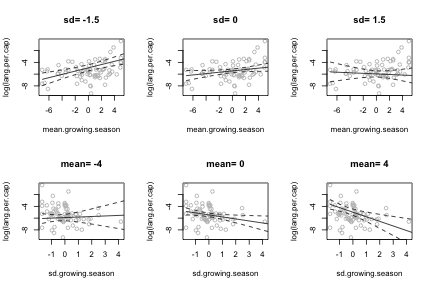
\includegraphics{lang-grow-fig} \begin{flushleft}
\ttfamily\noindent
\hspace*{\fill}\\
\hlstd{}\hlfunctioncall{par}\hlkeyword{(}\hlsymbol{op}\hlkeyword{)}\mbox{}
\normalfont
\end{flushleft}
\end{kframe}}
\end{knitrout}


The overall results support for the (vague) hypothesis that language diversity is effected by food security. 
From the correlational evidence presented here, however, the story is more complex due to an interaction between mean length and standard deviation of growing season.
The overall picture is shown in the triptych plots above.
Of the models considered, the model with this interaction is strongly favored.

The result is that for below average to average variability, increases in the mean growing season have the positive hypothesized effect. 
As variability increases, this effect weakens (top row of figure above).
For more variable seasons with average to above average length (bottom row), the effect of variability is is negative on language diversity. 

A mechanistic explanation is that stable, productive habitats permit local interactions and isolation of language, while variable habitats require broader ranges of interactions. 
The effect of variability is espeically strong when habitats are more productive (longer growing season).


The relationships picked out in the regression and described above can be seen to some extent in the raw data, visualized in the dot plots below: 

\begin{knitrout}
\definecolor{shadecolor}{rgb}{.97, .97, .97}{\color{fgcolor}\begin{kframe}
\begin{flushleft}
\ttfamily\noindent
\hlsymbol{g}{\ }\hlassignement{\usebox{\hlnormalsizeboxlessthan}-}{\ }\hlfunctioncall{ggplot}\hlkeyword{(}\hlsymbol{d.rc}\hlkeyword{)}\hspace*{\fill}\\
\hlstd{}\hlsymbol{g1}{\ }\hlassignement{\usebox{\hlnormalsizeboxlessthan}-}{\ }\hlsymbol{g}{\ }\hlkeyword{+}{\ }\hlfunctioncall{geom\usebox{\hlnormalsizeboxunderscore}point}\hlkeyword{(}\hlfunctioncall{aes}\hlkeyword{(}\hlsymbol{mean.growing.season}\hlkeyword{,}{\ }\hlfunctioncall{log}\hlkeyword{(}\hlsymbol{lang.per.cap}\hlkeyword{)}\hlkeyword{,}\hspace*{\fill}\\
\hlstd{}{\ }{\ }{\ }{\ }\hlargument{size}{\ }\hlargument{=}{\ }\hlsymbol{sd.growing.season}\hlkeyword{)}\hlkeyword{)}\hspace*{\fill}\\
\hlstd{}\hlsymbol{g1}\mbox{}
\normalfont
\end{flushleft}
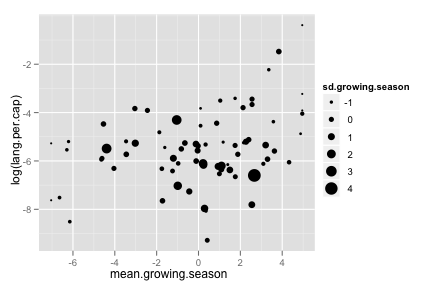
\includegraphics{gg-mean} \end{kframe}}
\end{knitrout}


\begin{knitrout}
\definecolor{shadecolor}{rgb}{.97, .97, .97}{\color{fgcolor}\begin{kframe}
\begin{flushleft}
\ttfamily\noindent
\hlsymbol{g2}{\ }\hlassignement{\usebox{\hlnormalsizeboxlessthan}-}{\ }\hlsymbol{g}{\ }\hlkeyword{+}{\ }\hlfunctioncall{geom\usebox{\hlnormalsizeboxunderscore}point}\hlkeyword{(}\hlfunctioncall{aes}\hlkeyword{(}\hlsymbol{sd.growing.season}\hlkeyword{,}{\ }\hlfunctioncall{log}\hlkeyword{(}\hlsymbol{lang.per.cap}\hlkeyword{)}\hlkeyword{,}\hspace*{\fill}\\
\hlstd{}{\ }{\ }{\ }{\ }\hlargument{size}{\ }\hlargument{=}{\ }\hlsymbol{mean.growing.season}\hlkeyword{)}\hlkeyword{)}\hspace*{\fill}\\
\hlstd{}\hlsymbol{g2}\mbox{}
\normalfont
\end{flushleft}
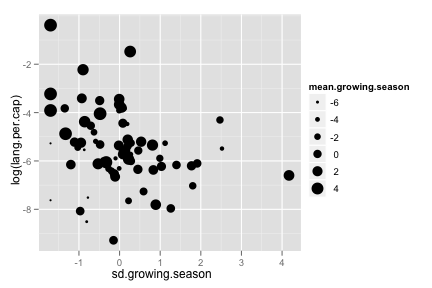
\includegraphics{gg-sd} \end{kframe}}
\end{knitrout}


\subsection*{Colophon}

\begin{knitrout}
\definecolor{shadecolor}{rgb}{.97, .97, .97}{\color{fgcolor}\begin{kframe}
\begin{flushleft}
\ttfamily\noindent
\hlfunctioncall{require}\hlkeyword{(}\hlsymbol{knitr}\hlkeyword{)}{\ }{\ }\hlcomment{\usebox{\hlnormalsizeboxhash}\usebox{\hlnormalsizeboxhash}\usebox{\hlnormalsizeboxhash}{\ }the{\ }package}\hspace*{\fill}\\
\hlstd{}\hlfunctioncall{knit}\hlkeyword{(}\hlfunctioncall{paste}\hlkeyword{(}\hlfunctioncall{getwd}\hlkeyword{(}\hlkeyword{)}\hlkeyword{,}{\ }\hlstring{"hw6ashander.Rnw"}\hlkeyword{,}{\ }\hlargument{sep}{\ }\hlargument{=}{\ }\hlstring{"/"}\hlkeyword{)}\hlkeyword{)}{\ }{\ }\hlcomment{\usebox{\hlnormalsizeboxhash}\usebox{\hlnormalsizeboxhash}{\ }to{\ }run}\hspace*{\fill}\\
\hlstd{}\hspace*{\fill}\\
\hlstd{}\hlcomment{\usebox{\hlnormalsizeboxhash}\usebox{\hlnormalsizeboxhash}{\ }to{\ }use{\ }all{\ }cores}\hspace*{\fill}\\
\hlstd{}\hlfunctioncall{require}\hlkeyword{(}\hlsymbol{snowfall}\hlkeyword{)}\hspace*{\fill}\\
\hlstd{}\hlfunctioncall{sfInit}\hlkeyword{(}\hlargument{parallel}{\ }\hlargument{=}{\ }\hlnumber{TRUE}\hlkeyword{,}{\ }\hlargument{cpus}{\ }\hlargument{=}{\ }\hlnumber{4}\hlkeyword{)}\hspace*{\fill}\\
\hlstd{}\hlfunctioncall{sfLibrary}\hlkeyword{(}\hlsymbol{rethinking}\hlkeyword{)}\hspace*{\fill}\\
\hlstd{}\hlfunctioncall{sfExportAll}\hlkeyword{(}\hlkeyword{)}\hspace*{\fill}\\
\hlstd{}\hlfunctioncall{sfStop}\hlkeyword{(}\hlkeyword{)}\mbox{}
\normalfont
\end{flushleft}
\end{kframe}}
\end{knitrout}



\end{document}
